\documentclass[aspectratio=169,11pt]{beamer}
\usepackage{beamertemplate}
% --- estilo de comandos (consistente con el resto del temario) ---
\newcommand{\cmd}[1]{\texttt{\color{uznavy}#1}}
\newcommand{\cmdbox}[1]{%
  \begin{center}%
  {\setlength{\fboxsep}{6pt}\colorbox{uzlav!40}{\parbox{0.88\linewidth}{\ttfamily\footnotesize #1}}}%
  \end{center}}
\usepackage{graphicx}
\usepackage{url}
\usepackage{textcomp}
\usepackage{eurosym}
\usepackage[normalem]{ulem}
\usepackage{ragged2e}
\usepackage{etoolbox}
\apptocmd{\itemize}{\justifying}{}{}
\AtBeginEnvironment{frame}{\justifying}

% Las secciones no actuales se muestran atenuadas al 30 %
\setbeamertemplate{section in toc shaded}[default][30]

% Repite el índice al empezar cada sección, resaltando la que comienza
\AtBeginSection[]{%
  \begin{frame}{Índice}
  \footnotesize
  \tableofcontents[currentsection]
  \end{frame}
}

\title[SSI -- Tema 2.1]{Footprinting y OSINT}
\subtitle{Seguridad en Sistemas Informáticos --- Tema 2.1}
\author{José Luis Martínez}
\institute{Universidad de Castilla-La Mancha}
\date{Curso 2026/27}

% --- build reproducible / metadatos limpios ---
\pdfinfoomitdate=1
\pdftrailerid{}
\pdfsuppressptexinfo=-1

\begin{document}

\begin{frame}[plain]\titlepage\end{frame}

\begin{frame}{Índice}
\small
\tableofcontents
\end{frame}

\begin{frame}{Taxonomía de un Ataque}
\begin{center}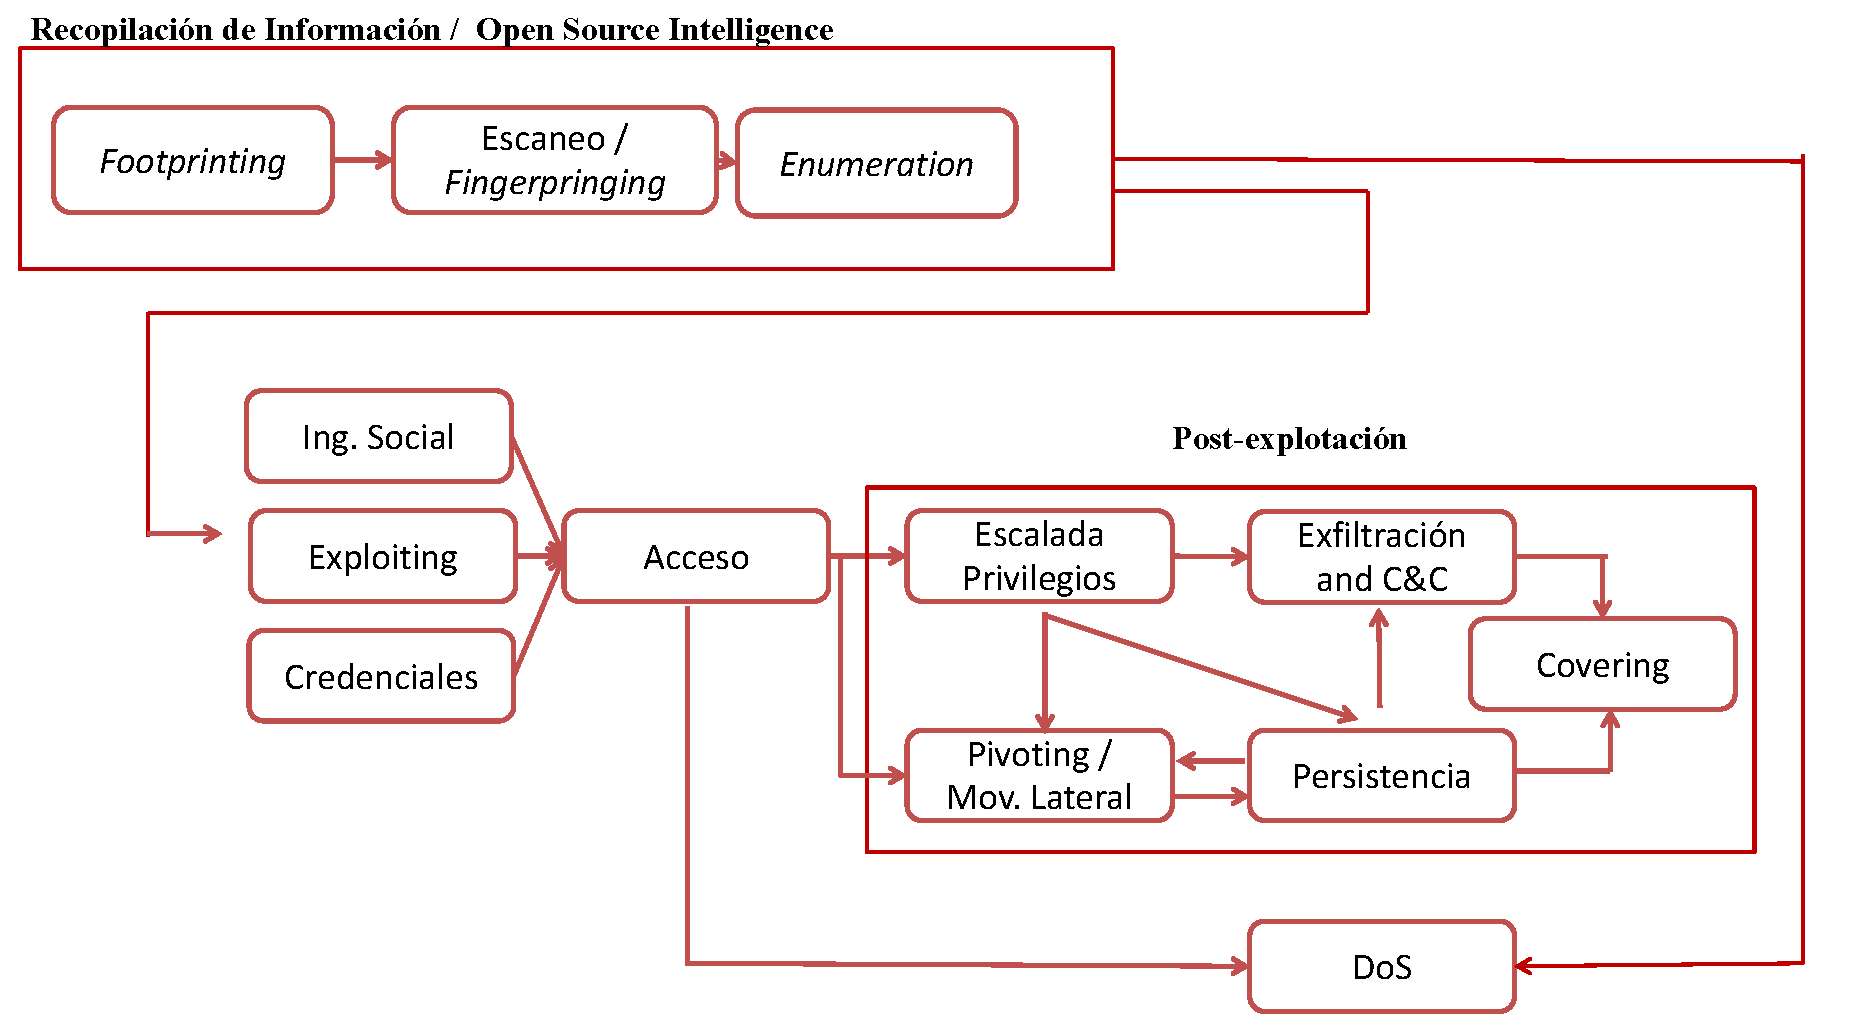
\includegraphics[width=\textwidth,height=0.82\textheight,keepaspectratio]{img/taxonomia-ataque.pdf}
\end{center}
\end{frame}



\section{Introducción}

\begin{frame}{Introducción}
\footnotesize
¿Qué es un ejercicio de red Team?
  \begin{itemize}
  \item Son acciones que intentan comprometer la empresa por varios vectores de entrada, incluidos vectores como ingeniería social.
  \item Una vez llevada a cabo la intrusión, se intentan comportar como lo haría un atacante, buscando persistencia, pivotando a máquinas internas, Domain Controller, etc
  \item Es asumir que tu empresa va a ser atacada, y con estos ejercicios puedes ver cómo se comporta ésta frente a ataques o qué información puede ser accedida / robada por un atacante
  \item Muy poca gente de la empresa conoce que se está realizando este ejercicio
  \item Suelen seguir la siguiente metodología, que puede ser modificada en caso de hacer uso del framework TIBER-EU
  \end{itemize}
\vfill
\begin{center}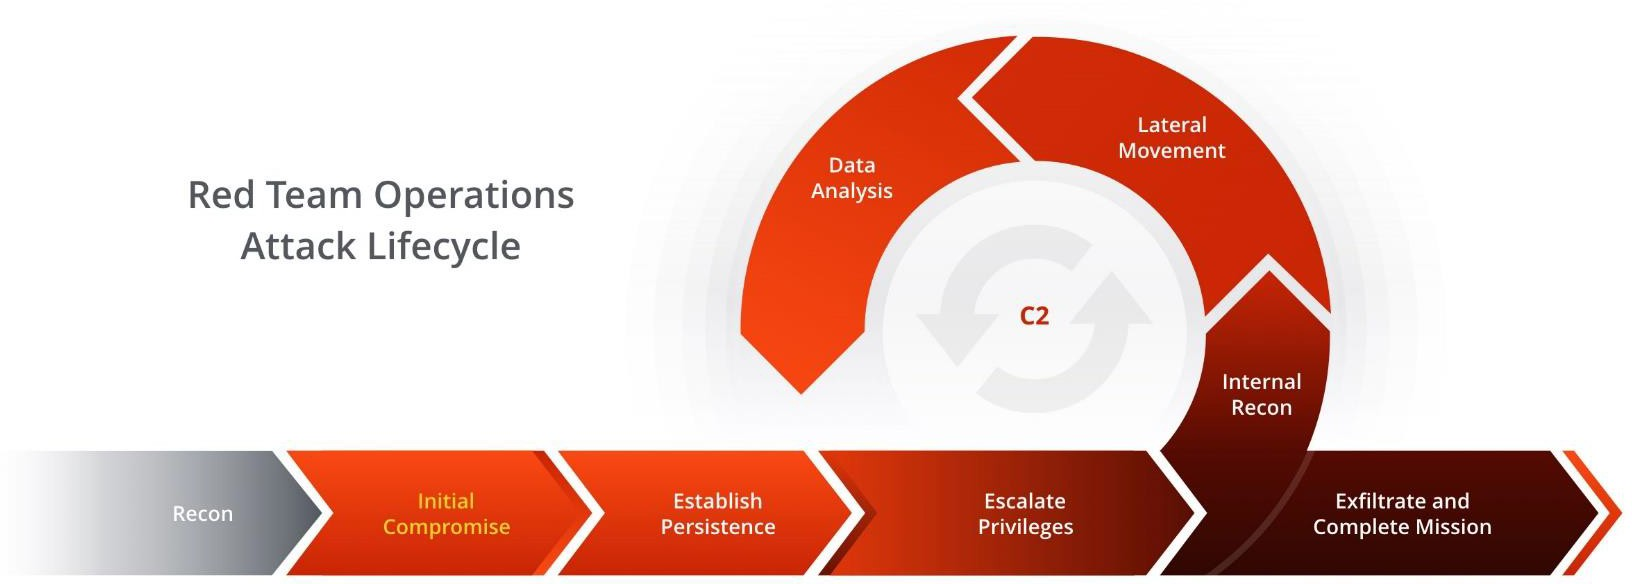
\includegraphics[width=0.80\textwidth,height=0.30\textheight,keepaspectratio]{img/sl006.jpg}
\end{center}
\end{frame}

\begin{frame}[allowframebreaks]{Introducción}
\small
  \begin{itemize}
  \item Se diferencia de una auditoría de vulnerabilidades, en la que se suele lanzar un escáner (Nessus, por ejemplo) para ver los fallos
  \item A diferencia de una pentesting, que el objetivo es encontrar una vulnerabilidad crítica, de las que permitan la ejecución remota de código y la intrusión. Nota: No todas las vulnerabilidades reportadas dan lugar a una ejecución remota de código
  \item Un ejercicio de red team es mucho más completo, simula un ataque real, de un enemigo con muchos recursos, lo que podría ser un Advanced Persistent Threat (APT)
  \end{itemize}
\end{frame}

\begin{frame}[allowframebreaks]{Introducción}
\small
¿Qué es el footprinting?
  \begin{itemize}
  \item Se identifica con la fase de `recopilación/obtención de información' dentro del proceso de auditoria, y su principal objetivo es obtener información general de la entidad a ser auditada, así como el conjunto de activos sobre los que serán desarrollados pruebas posteriormente.
  \item Esta fase puede no cobra mucho sentido según que tipo de auditorias, y ser especialmente relevante en otras como los ejercicios Red Team
  \end{itemize}
\end{frame}

\begin{frame}[allowframebreaks]{Introducción}
\small
Mediante el uso de acciones mayoritariamente pasivas, que no permitan la identificación del equipo, se desarrollaran las pruebas con el objetivo de buscar información como:

\begin{itemize}
  \item Empresas que conforman el objetivo
  \item Infraestructura objetivo (perímetro, wifi, \dots{})
  \item Información sobre la red interna
  \item Información sensible
  \item Usuarios internos \& Leaks de usuarios y/o contraseñas
  \item Número de teléfono
  \item Geolocalización
  \item Whois, DNS
  \item Tecnologías usadas, sistemas, aplicaciones
  \end{itemize}
\end{frame}

\begin{frame}[allowframebreaks]{Introducción}
\small
  \begin{itemize}
  \item Se podría decir que esta fase sirve para identificar al detalle los activos que vamos a auditar, para posteriormente, analizar la información e identificar posibles vulnerabilidades que puedan permitir algún tipo de acción en el activo.
  \item Dos tipos:
    \begin{itemize}

  \item Pasivo: en el que no se interactúa con el objetivo (Ejemplo, a través de buscadores)
  \item Activo: en el que si se interactúa (Ejemplo, a través de herramientas como dnsmap, etc)
  \item \dots{}anónimo?
    \end{itemize}

  \end{itemize}
\end{frame}


\section{Operadores de búsqueda avanzados}

\begin{frame}[allowframebreaks]{Operadores de búsqueda avanzados}
\small
   El objetivo es usar buscadores públicos para encontrar información sensible útil para un posterior ataque

  \begin{itemize}
  \item Algunos de los principales operadores de búsqueda son los siguientes:
    \begin{itemize}
  \item site: Permite hacer búsquedas por un determinado dominio.
  \item intitle / allintitle: Permite hacer búsquedas en el titulo de la web.
  \item inurl / allinurl: Permite hacer búsquedas en la URL indexada.
  \item intext / allintext: Permite hacer búsquedas en el propio texto de la web.
  \item ext / filetype: Permite hacer búsquedas por una determinada extensión o tipo de fichero (comprobado por Google) respectivamente.
  \item `-': Permite negar cualquiera de los anteriores operadores.
  \item Existen mas operadores de búsqueda avanzados, pero estos son sin duda los mas útiles, potentes y comúnmente utilizados.
  \end{itemize}
  \end{itemize}
\end{frame}

\begin{frame}[allowframebreaks]{Operadores de búsqueda avanzados}
\small
  \begin{itemize}
  \item Ejemplos: \href{http://www.googleguide.com/advanced_operators_reference.html\#cache}{Guía completa de operadores:}
  \end{itemize}
\begin{center}
\includegraphics[width=0.72\textwidth,height=0.58\textheight,keepaspectratio]{img/sl014.png}
\end{center}
\end{frame}

\begin{frame}{Operadores de búsqueda avanzados}
\small
  \begin{itemize}
  \item \href{https://www.exploit-db.com/google-hacking-database}{Google Hacking DataBase} (GHDB)
  \item Es un proyecto donde la gente comparte sus `dorks' personalizados, nombre que se le da a las búsquedas avanzas que hacen uso de operadores para conseguir una determinada información.
  \item Herramientas:
    \begin{itemize}
    \item \href{https://github.com/m3n0sd0n4ld/uDork}{uDork}
    \item \href{https://github.com/m3n0sd0n4ld/GooFuzz}{GooFuzz}
    \item \href{https://github.com/six2dez/dorks_hunter}{Dorks\_hunter}
    \end{itemize}
  \end{itemize}
\vfill
\begin{center}
\includegraphics[width=0.6\textwidth,height=0.4\textheight,keepaspectratio]{img/sl015.png}
\end{center}
\end{frame}

\begin{frame}[allowframebreaks]{Operadores de búsqueda avanzados}
\small
Servicios online
  \begin{itemize}
  \item La mayoría de organizaciones, y mejor dicho, empleados, hacen uso de herramientas y aplicaciones en Internet donde almacenan información de la entidad. Es interesante analizar mediante algunos dorks estos servicios, en busca de posible información como: usuarios y credenciales, dominios y direcciones IP internas, detalles de infraestructura, etcétera.
  \item Algunos de los servicios que podrían ser analizados son:
  \begin{itemize}

  \item \href{https://pastebin.com/}{Pastebin}
  \item \href{https://github.com/}{GitHub}
  \item \href{https://trello.com/}{Trello}
    \end{itemize}

  \item Esta información puede ser muy útil para encontrar un vector de acceso.
  \end{itemize}
\end{frame}

\begin{frame}[allowframebreaks]{Operadores de búsqueda avanzados}
\small
  \begin{itemize}
  \item En caso de querer utilizar técnicas de Google Hacking de forma común, es posible crear búsquedas personalizadas, que se encarguen de buscar en algunos de los servicios descritos previamente. Un ejemplo es:
  \begin{itemize}

  \item https://cse.google.com/cse/all
    \end{itemize}

  \item Existen servicios como Github donde es posible encontrar información interesante, y además poder hacer búsquedas simples pero potentes como las siguientes, que permiten buscar por organización, y posteriormente por usuarios de dicha organización.
  \begin{itemize}
  \item https://github.com/orgs/[organizacion]/people
  \item https://api.github.com/users/[usuarios]/events/public
 \end{itemize}
  \item En cualquier caso, también existen herramientas que automatizan esta labor: \href{https://github.com/trufflesecurity/trufflehog}{TruffleHog}, \href{https://github.com/gitleaks/gitleaks}{Gitleaks} (escaneo de secretos en repos) o \textbf{GitHub dorks} para localizar credenciales (\cmd{\textquotedbl{}password\textquotedbl{} org:empresa}, \cmd{filename:.env}, \cmd{extension:pem})
  \end{itemize}
\end{frame}

\begin{frame}{Ejercicio}
\small
\begin{center}
\includegraphics[width=0.45\textwidth,height=0.4\textheight,keepaspectratio]{img/sl020.jpg}
\end{center}
\vspace{0.5em}
  \begin{itemize}
  \item Realiza consultas ''google hacking'' frente a una organización a tu elección para encontrar información sensible de ésta
  \item Utiliza la herramienta dorks\_hunter:
    \begin{itemize}
    \item git clone https://github.com/six2dez/dorks\_hunter
    \item pip3 install -r requirements.txt \# Python 3.8+ y xnldorker
    \item python3 dorks\_hunter.py -d objetivo.com -o resultados.txt
    \end{itemize}
  \end{itemize}
\vfill
\end{frame}

\begin{frame}{Ejercicio}
\small
\begin{center}
\includegraphics[width=0.45\textwidth,height=0.4\textheight,keepaspectratio]{img/sl021.jpg}
\end{center}
\vspace{0.5em}
Resuelve esta room de TryHackme:
  \begin{itemize}
  \item \href{https://tryhackme.com/r/room/googledorking}{googledorking}
  \end{itemize}
\end{frame}

\begin{frame}[allowframebreaks]{Operadores de búsqueda avanzados}
\small
Bibliorafía:
  \begin{itemize}
  \item \href{https://vimeo.com/24506384}{Charla sobre hacking con buscadores}
  \item \href{https://www.youtube.com/watch?v=VNhXZvW7t9Q}{Charla Google hacking}
  \item \href{https://www.osi.es/es/actualidad/blog/2017/06/14/buscadores-que-no-invaden-nuestra-privacidad}{Buscadores que no invaden nuestra privacidad}
  \item Ejemplos de uso:
    \begin{itemize}
    \item Caso 1: \href{https://hacking-etico.com/2011/07/20/se-hacking-etico-google-hacking-parte-1/}{parte1}, \href{https://hacking-etico.com/2011/07/25/se-hacking-etico-google-hacking-\%e2\%80\%93-parte-2/}{parte2}, \href{https://hacking-etico.com/2012/05/05/se-hacking-etico-google-hacking-parte-3/}{parte3}
    \item Caso 2: \href{https://fwhibbit.es/hacking-con-buscadores-i-leak-information}{parte1}, \href{https://fwhibbit.es/hacking-con-buscadores-ii-preguntando-las-contrasenas-a-los-buscadores}{parte2}, \href{https://fwhibbit.es/hacking-con-buscadores-iii-metalocalizando-rutas}{parte3}, \href{https://fwhibbit.es/hacking-con-buscadores-iv-buscando-vulnerabilidades-y-objetivos}{parte4}
    \item Caso 3: \href{https://fwhibbit.es/hacking-con-buscadores-episodio-i-la-amenaza-del-search}{parte1}, \href{https://fwhibbit.es/hacking-con-buscadores-episodio-ii-el-ataque-de-inyecciones-sql}{parte2}, \href{https://fwhibbit.es/hacking-con-buscadores-episodio-iii-la-venganza-de-las-shells}{parte3}, \href{https://fwhibbit.es/hacking-con-buscadores-episodio-iv-una-nueva-esperanza-al-internet-de-las-cosas}{parte4}, \href{https://fwhibbit.es/hacking-con-buscadores-episodio-v-el-internet-of-things-contraataca}{parte5}
    \item \href{https://www.elladodelmal.com/2010/02/google-hacking-inurl-ext-y-filetype.html}{Caso 4:}
    \item \href{https://www.elladodelmal.com/2014/05/buscar-bugs-de-heartbleed-en-well-known.html}{Caso 5:}
    \item \href{https://hacking-etico.com/2013/12/13/tus-documentos-en-la-nube-indexados/}{Caso 6:}
    \item \href{https://hacking-etico.com/2012/08/29/encontrando-htaccess-y-htpasswd-antiguos-con-google-hacking/}{Caso 7:}
    \item Caso 8: \href{https://www.elladodelmal.com/2010/06/buscadores-como-arma-de-destruccion.html}{parte1}, \href{https://www.elladodelmal.com/2010/03/buscadores-como-arma-de-destruccion.html}{parte2}, \href{https://www.elladodelmal.com/2010/05/buscadores-como-arma-de-destruccion.html}{parte3}
    \end{itemize}
  \end{itemize}
\end{frame}

\begin{frame}[allowframebreaks]{Operadores de búsqueda avanzados}
\small
  \begin{itemize}
  \item Google Dorks: Ejemplos Prácticos:
    \begin{itemize}

  \item Credenciales y claves API en repositorios
  \item site:github.com \textquotedbl{}password\textquotedbl{} OR \textquotedbl{}api\_key\textquotedbl{} ext:env
  \item site:pastebin.com \textquotedbl{}smtp\_password\textquotedbl{} OR \textquotedbl{}db\_password\textquotedbl{}
  \item $\rightarrow$ Muchos desarrolladores suben accidentalmente ficheros .env con credenciales reales
      \end{itemize}

  \item Paneles de administración expuestos
      \begin{itemize}

  \item site:empresa.com intitle:\textquotedbl{}admin panel\textquotedbl{} OR intitle:\textquotedbl{}login\textquotedbl{}
  \item inurl:\textquotedbl{}/wp-admin/setup-config.php\textquotedbl{} site:empresa.com
        \end{itemize}

  \item Documentos internos filtrados
        \begin{itemize}

  \item site:empresa.com filetype:pdf \textquotedbl{}confidencial\textquotedbl{} OR \textquotedbl{}uso interno\textquotedbl{}
  \item site:empresa.com filetype:xls \textquotedbl{}usuario\textquotedbl{} OR \textquotedbl{}contraseña\textquotedbl{} OR \textquotedbl{}password\textquotedbl{}
  \item $\rightarrow$ exploit-db.com/google-hacking-database agrupa miles de dorks categorizados
          \end{itemize}

  \end{itemize}
\end{frame}

\section{Filtraciones de datos}

\begin{frame}[allowframebreaks]{Filtraciones de datos}
\small
  \begin{itemize}
  \item Adicionalmente también es recomendable revisar cuales son los dominios utilizados por los servidores de correo de la entidad, y buscar si hubiera algún usuario interno que apareciera en leaks públicos recientes.
  \item Esto permite obtener direcciones de correo y posibles credenciales, aunque lo mas habitual es que estas no sean válidas en el dominio interno.
  \item En cualquier caso, pueden servir para identificar usuarios que siguen patrones en las contraseñas, o posteriormente utilizar las direcciones de correo para crear ataques de fuerza bruta contra servicios que autentiquen contra el dominio interno como la VPN o el correo.
  \item A veces los leaks los encontramos en la Deep web o en foros rusos
  \end{itemize}
\end{frame}

\begin{frame}[allowframebreaks]{Filtraciones de datos}
\small
  \begin{itemize}
  \item Un ejemplo podría ser la web haveibeenpwn que, a partir de un correo, nos dice si éste esta asociado a servicios que han tenido leks de información y es posible que la password este leakeada
  \item Otras webs son isleaked o dehashed
  \item Herramientas:
    \begin{itemize}

  \item \href{https://github.com/loseys/Oblivion}{Oblivion}
  \item \href{https://github.com/Telefonica/HashCheck}{HashCheck}
  \item \href{https://github.com/thewhiteh4t/pwnedOrNot}{pwnedOrNot}
  \item \href{https://github.com/daab0x/EMAGNET}{EMAGNET}
    \end{itemize}


  \end{itemize}
\end{frame}

\begin{frame}[allowframebreaks]{Filtraciones de datos}
\small
  \begin{itemize}
  \item Aunque existen servicios expuestos en Internet que almacenan leaks, es muy común que estos sean cerrados. Aun así, alguna de las herramientas que mejor funciona es Pwndb, que hace uso de ciertos servicios en TOR con esta información. 
  \item Esta url es una copia en internet del dominio en Tor:
  \item \href{https://pwndb2am4tzkvold.onion.ws/}{https://pwndb2am4tzkvold.onion.ws/}
  \item LeakedPasswordDatabase - Encontrar contraseñas abiertas en internet
   \begin{itemize}

  \item http://breachdbsztfykg2fdaq2gnqnxfsbj5d35byz3yzj73hazydk4vq72qd.onion/Tips
  \item http://cryptbbtg65gibadeeo2awe3j7s6evg7eklserehqr4w4e2bis5tebid.0ni0 - cryptbb
\end{itemize}
  \item Otra opción también interesante sería el uso de APIs en servicios públicos a esas web en la Deep web:
  \begin{itemize}

  \item https://leak-lookup.com/databases
  \item https://www.dehashed.com/data
\end{itemize}
  \end{itemize}
\end{frame}

\begin{frame}[allowframebreaks]{Filtraciones de datos}
\small
  \begin{itemize}
  \item Servicios para encontrar brechas de seguridad con filtraciones de datos sensibles:
    \begin{itemize}
 
  \item https://cracking.org
  \item https://z-lib.is
  \end{itemize}

  \item Actual enlace a la librería mas grande de internet, llena de recursos libres y miles de libros de pago, acceder con VPN muchos ISP bloquean el acceso
  \begin{itemize}
  \item https://leakbase.io
  \item https://leakedbb.io
  \item https://nulled.to
  \item https://xss.is
  \item https://intelx.io/
  \item https://nuclearleaks.com/
  \item https://haveibeensold.app/
  \item https://www.dehashed.com/
  \item https://mypwd.io/
  \item https://leakcheck.net/

  \end{itemize}

  \end{itemize}
\end{frame}

\begin{frame}{Filtraciones de datos}
\small
\begin{columns}[c]
\begin{column}{0.60\textwidth}
  \begin{itemize}
  \item Google ha lanzado una herramienta para comprobar si tú email se ha filtrado en la DarkWeb. Se entra desde \href{https://one.google.com}{one.google.com} y pulsando en el botón de \textquotedbl{}Informe sobre DarkWeb\textquotedbl{} nos dirá el sitio en el que se robó el dato.
  \end{itemize}
\end{column}
\begin{column}{0.38\textwidth}
\begin{center}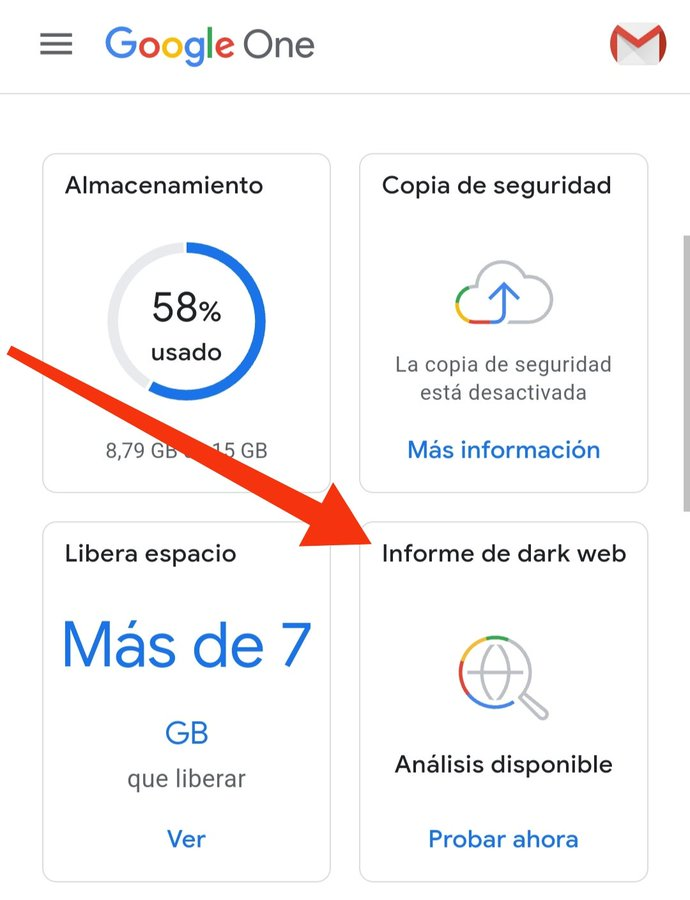
\includegraphics[width=\textwidth,height=0.85\textheight,keepaspectratio]{img/sl027.jpg}
\end{center}
\end{column}
\end{columns}
\end{frame}

\begin{frame}[allowframebreaks]{Filtraciones de datos}
\small
Brechas Históricas Relevantes
  \begin{itemize}
  \item RockYou2024 (2024) --- La mayor filtración conocida
  \begin{itemize}
  \item 10.000 millones de contraseñas en texto claro en un foro de hacking
  \item $\rightarrow$ Permite ataques de credential stuffing a escala masiva
    \end{itemize}

  \item LinkedIn (2021) --- 700 millones de perfiles
    \begin{itemize}

  \item Datos raspados: nombre, email, teléfono, empresa, cargo, URL de perfil
  \item $\rightarrow$ Base perfecta para spear phishing dirigido a ejecutivos (BEC fraud)
      \end{itemize}

  \item Collection \#1 (2019)
    \begin{itemize}

  \item 773 millones de emails + 21 millones de contraseñas únicas en texto plano
  \item Verificable en haveibeenpwned.com --- referencia habitual en auditorías de contraseñas
        \end{itemize}

  \item Adobe (2013) --- 153 millones de cuentas
      \begin{itemize}

  \item Contraseñas cifradas con DES (roto): permite cracking offline rápido
  \item $\rightarrow$ Revela patrones: usuarios que usan la misma contraseña en múltiples servicios
  
          \end{itemize}

  \end{itemize}
\end{frame}

\section{Correos electrónicos}

\begin{frame}[allowframebreaks]{Correos electrónicos}
\small
  \begin{itemize}
  \item Existen herramientas que, a partir de búsquedas en Internet, de manera pasiva, encuentran correos (emails) validos de la organización objetivo. Por ejemplo:
  \begin{itemize}

  \item Buscando en foros usuarios registrados con ese mail
  \item Servicios de google registrados
  \item RRSS como LinkedIn, Facebook, people123, etc

  \end{itemize}
  \item Herramientas:
  \begin{itemize}

  \item \href{https://github.com/laramies/theHarvester}{theHarvester}
  \item \href{https://hunter.io/}{Hunter.io}
  \item \href{https://epieos.com/}{Epieos}
    \end{itemize}
  \item Herramientas para obtener información a partir de un correo electrónico
    \begin{itemize}

  \item \href{https://github.com/Quantika14/email-osint-ripper}{Ripper (EO-Ripper)}
  \item \href{https://github.com/mxrch/GHunt}{GHunt}
  \item \href{https://github.com/megadose/holehe}{holehe}
  \item \href{https://www.linkedin.com/posts/vicentegarrigues-trenor_osint-cybersecurity-emailosint-ugcPost-7336529048434606080-MccL/}{ZEHEF}
  \item \href{https://www.linkedin.com/posts/carlos-bartels-66a60763_osint-cybersecurity-threatintelligence-activity-7298811240082989057-o7pd/}{Mosint}
  \end{itemize}
  \end{itemize}
\end{frame}

\begin{frame}[allowframebreaks]{Correos electrónicos}
\small
Verificación y Descubrimiento de Correos: Toolkit Completo
  \begin{itemize}
  \item Herramientas para descubrir, validar y enriquecer información sobre correos:
  \item Descubrimiento de correos por dominio
  \begin{itemize}

  \item phonebook.cz --- busca emails, dominios e IPs asociados a una organización
  \item intelx.io --- motor de inteligencia con acceso a filtraciones indexadas
  \item intelx.io/?s=uclm.es $\leftarrow$ ejemplo: buscar exposición del dominio uclm.es
  \end{itemize}

  \item Verificación de existencia de un email
  \begin{itemize}

  \item email-checker.net --- verifica si un email es válido sin enviar mensaje
  \item verifyemailaddress.org --- validación SMTP sin revelar la consulta
  \item verifyemailaddress.org/email-validation
  \item Flujo recomendado en auditoría
  \item $\rightarrow$ 1. Descubrir emails con phonebook.cz / Hunter.io / TheHarvester
  \item $\rightarrow$ 2. Validar con email-checker o verifyemailaddress
  \item $\rightarrow$ 3. Cruzar con intelx.io / HaveIBeenPwned para detectar credenciales filtradas
  \end{itemize}

\end{itemize}
\end{frame}

\begin{frame}{Ejercicio}
\small
\begin{center}
\includegraphics[width=0.45\textwidth,height=0.4\textheight,keepaspectratio]{img/sl030.jpg}
\end{center}
\vspace{0.5em}
  \begin{itemize}
  \item Para la misma organización del ejercicio anterior, encuentra correos de trabajadores y, para algunos de ellos comprueba si sus contraseñas pueden estar comprometidas
  \end{itemize}
\end{frame}

\section{Enumeración de usuarios}

\begin{frame}[allowframebreaks]{Enumeración de usuarios}
\small
  \begin{itemize}
  \item Independientemente del número de usuarios que se obtengan en Leaks siempre es interesante obtener el mayor número de empleados y sus direcciones de correo.
  \item Existen scripts que permiten automatizar esta tarea, haciendo búsquedas sobre LinkedIn en base a la organización que haya sido definida.
  \item Herramientas:
    \begin{itemize}

  \item \href{https://github.com/vaguileradiaz/tinfoleak}{Tinfoleak} (Python2)
  \item \href{https://github.com/vysecurity/LinkedInt}{LinkedInt}
  \item DataHunter
  \item \href{https://github.com/m8sec/CrossLinked}{CrossLinked}: python3 crosslinked.py -f '\{first\}.\{last\}@bbva.com' BBVA
  \end{itemize}
  \end{itemize}
\end{frame}

\begin{frame}{Ejercicio}
\small
\begin{center}
\includegraphics[width=0.45\textwidth,height=0.4\textheight,keepaspectratio]{img/sl032.jpg}
\end{center}
\vspace{0.5em}
  \begin{itemize}
  \item Utiliza herramientas tipo crosslinked o data-hunter para buscar usuarios de una organización objetivo
  \end{itemize}
\end{frame}

\begin{frame}{Enumeración de usuarios}
\footnotesize
Enumeración de usuarios en diferentes RRSS
\begin{columns}[c]
\begin{column}{0.78\textwidth}
  \begin{itemize}
  \item \href{https://netbootcamp.org/facebook.html}{Facebook}
    \item Twitter
      \begin{itemize}
      \item \href{https://tweetbeaver.com/}{Tweetbeaver}
      \item \href{https://socialbearing.com/}{Socialbearing}
      \item Tmap
      \item \href{https://foller.me/}{Foller.me}
      \item \href{https://www.allmytweets.net/connect/}{Allmytwitts}
      \item \href{https://followerwonk.com/}{Followerwonk}
      \item \href{https://tinfoleak.com/}{Tinfoleak}
      \end{itemize}
    \item \href{https://github.com/sc1341/InstagramOSINT}{Instagram}
      \begin{itemize}
      \item Análisis en Instagram: \href{https://ciberpatrulla.com/analisis-instagram-osint/}{Leer}
      \item \href{https://www.flu-project.com/2019/07/spiderfoot-mucho-mas-que-lejos-de-casa.html?m=1&s=03}{Scylla}
      \item \href{https://derechodelared.com/osintgram-osint-instagram/}{Osintgranm}
      \end{itemize}
  \item Para chequear usuarios activos en cualquier red social -> \href{https://checkusernames.com/}{checkusername} y \href{https://namechk.com/}{namecheck}
  \end{itemize}
\end{column}
\begin{column}{0.20\textwidth}
\begin{center}
\includegraphics[width=\textwidth,height=0.5\textheight,keepaspectratio]{img/sl033.jpg}
\end{center}
\end{column}
\end{columns}
\end{frame}

\begin{frame}[allowframebreaks]{Enumeración de usuarios}
\small
  \begin{itemize}
  \item \href{https://sherlock-project.github.io/}{Sherlock proyect}
    \begin{itemize}
    \item \href{https://ginseg.com/comunidad/investigar-por-nombre-de-usuario/userrecon-py-localiza-perfiles-sociales-a-partir-de-nombres-de-usuario/}{Userrecon}
    \item \href{https://github.com/Quantika14/osint-suite-tools}{Quantika14}
    \item \href{https://reaper.social/}{reaper}
    \item \href{https://hakin9.org/blackbird-an-osint-tool-to-search-for-accounts-by-username-in-social-networks/}{Blackbird}
    \item \href{https://github.com/soxoj/maigret}{Maigret} --- fork de Sherlock ($>$3000 sitios) que además extrae datos del perfil
    \item \href{https://whatsmyname.app/}{WhatsMyName} --- enumeración de \emph{usernames} (web y CLI)
    \end{itemize}
  \item Herramienta para listar usuarios (y contraseñas) en organizaciones que usan office 365:
    \begin{itemize}
    \item \href{https://www.blackhatethicalhacking.com/tools/go365/}{Go365}
    \end{itemize}
  \item Ver \href{https://www.youtube.com/watch?v=t1nw1uLF9L4}{video}
  \end{itemize}
\end{frame}

\begin{frame}[allowframebreaks]{Enumeración de Usuarios}
\small
  \begin{itemize}
  \item Una vez se cuenta con los empleados identificados, es común intentar identificar cuales de ellos son cuentas reales y cuales no, de cara a posteriores ataques como el desarrollo de fuerza bruta.
  \item Para ello se puede hacer uso de diferentes técnicas:
  \begin{itemize}

  \item Identificación de enumeración de usuarios en paneles web corporativos
  \item Identificación de Office365 y desarrollo de pruebas
  \item Envío de correos (es agresivo)
  \end{itemize}
  \end{itemize}
\end{frame}

\begin{frame}[allowframebreaks]{Enumeración de Usuarios}
\small
\href{https://fwhibbit.es/osint-parte-i-todo-lo-que-sabe-google-de-nosotros}{¿y personas? Puedo buscar personas en Internet}
  \begin{itemize}
  \item Herramientas:
    \begin{itemize}
    \item \href{https://webmii.com/}{Webmii}
    \item \href{https://pipl.com/}{Pipl}
    \item \href{https://www.spokeo.com/}{spokeo}
    \end{itemize}
  \item Crear personas falsas --para ingeniería social-
    \begin{itemize}
    \item Generación se usuario aleatorios con \href{https://randomuser.me/}{randomuser}
    \item Generación de nombres con \href{https://www.name-generator.org.uk/}{name-generator} o \href{https://www.fakenamegenerator.com/}{fakenamegenerator} o \href{https://randomwordgenerator.com/name.php}{randomwordgenerator}
    \item Generación de id aleatorios con \href{https://www.elfqrin.com/fakeid.php}{elfgrin}
    \item Imágenes de personas ficticias con \href{https://thispersondoesnotexist.com/}{thispersondoesnotexit}
    \item \href{https://www.flu-project.com/2019/11/generando-imagenes-mediante-rosebud-ai.html}{Lectura}
    \end{itemize}
  \item Lectura Complementaria:
    \begin{itemize}
    \item Caso de Uso: \href{https://fwhibbit.es/harvey-v1-2-analisis-de-un-objetivo-parte-i}{parte1}, \href{https://fwhibbit.es/harvey-v1-2-vigilancia-y-monitorizacion-en-twitter-parte-ii}{parte2}, \href{https://www.youtube.com/watch?v=52bqF0coBfU}{footprinting e ingeniería social}
    \end{itemize}
  \end{itemize}
\end{frame}

\begin{frame}[allowframebreaks]{Enumeración de Usuarios}
  Usuarios -- Correos -- Personas
\begin{center}
\includegraphics[width=0.72\textwidth,height=0.58\textheight,keepaspectratio]{img/sl037.png}
\end{center}
\end{frame}

\section{Tecnologías y sistemas}

\begin{frame}[allowframebreaks]{Tecnologías y sistemas}
\small
  \begin{itemize}
  \item Se puede recopilar información de la infraestructura de la compañía a partir de los puesto de trabajo que oferta en webs como:
    \begin{itemize}

  \item LinkedIn
  \item InfoJobs
\end{itemize}
  \item Por ejemplo, si buscan programador PHP o si buscan expertos en Centos.
  
  \item Herramientas para determinar el sistema operativo usando por la organización objetivo:
    \begin{itemize}
  \item \href{https://sitereport.netcraft.com/}{Netcraft} (Site Report)
 
\end{itemize}
  \end{itemize}
\end{frame}

\begin{frame}[allowframebreaks]{Tecnologías y sistemas}
\small
  \begin{itemize}
  \item Herramienta para búsquedas de dispositivos conectados tales como routers, servidores, IoT y con variedad de filtros
    \begin{itemize}
  \item \href{https://www.shodan.io/}{Shodan.io}
  \end{itemize}

  \item También identifica vulnerabilidades de forma pasiva
  \item Hay otro parámetro muy interesante que es buscar por el hash del favicon que permite buscar servicios web predeterminados como apache, jenkis, tomcat, etc...

  \item Ejemplos
  \begin{itemize}

  \item nmap en Shodan: smap
    \end{itemize}


  \item \href{https://search.censys.io/}{Censys.io}

  \item Buscar personas mediante Shodan con banner grabbing
  \item Cámaras:
 \begin{itemize}

  \item \href{http://www.insecam.org/}{insecam}
  \item \href{https://www.linkedin.com/posts/vicentegarrigues-trenor_cybersecurity-hackingaeztico-osint-ugcPost-7340848658659045376-mFBu/}{CamXploit} --- descubre cámaras/CCTV IP expuestas
  \end{itemize}

  \end{itemize}
\end{frame}

\begin{frame}{Tecnologías y sistemas}
\footnotesize
  \begin{itemize}
  \item También existe una herramienta en línea de comandos que hace consultas a shodan:
    \begin{itemize}
    \item \href{https://www.linkedin.com/posts/viehgroup_shodan-pentesting-guide-ugcPost-7130438265106513920-_THI/}{shodan}
    \end{itemize}
  \item Bibliografía:
    \begin{itemize}
    \item \href{https://www.elladodelmal.com/2014/01/shondan-proyectores-webcams-y-backups.html}{Caso de uso 1}
    \item \href{https://www.elladodelmal.com/2014/01/shondan-proyectores-webcams-y-backups.html}{Caso de uso 2}
    \item \href{https://www.elladodelmal.com/2011/06/es-seguro-mi-joomla-o-mi-wordpress.html}{Caso de uso 3}
    \item \href{https://www.elladodelmal.com/2011/06/es-seguro-mi-joomla-o-mi-wordpress.html}{Caso de uso 4}
    \item \href{https://www.elladodelmal.com/2012/10/donde-meto-mi-webshell-metodos.html}{Caso de uso 5}
    \item \href{https://www.elladodelmal.com/2013/04/buscar-sitios-web-con-applets-java.html}{Caso de uso 6}
    \item \href{https://www.elladodelmal.com/2010/05/shodan-y-ataques-telefonia-voip.html}{Caso de uso 7}
    \end{itemize}
  \end{itemize}
\vfill
\begin{center}
\includegraphics[width=0.8\textwidth,height=0.32\textheight,keepaspectratio]{img/sl039.png}
\end{center}
\end{frame}

\begin{frame}[allowframebreaks]{Tecnologías y sistemas}
\small
Búsquedas Útiles en Auditorías Reales:
  \begin{itemize}
  \item Sistemas vulnerables a CVEs conocidos:
    \begin{itemize}

  \item vuln:CVE-2021-44228 $\leftarrow$ Sistemas aún vulnerables a Log4Shell
  \item product:\textquotedbl{}Apache httpd\textquotedbl{} version:\textquotedbl{}2.4.49\textquotedbl{} $\leftarrow$ Path Traversal (CVE-2021-41773)
  \end{itemize}
  
  \item Cámaras IP y dispositivos IoT sin autenticación
    \begin{itemize}

  \item has\_screenshot:true port:554 $\leftarrow$ Cámaras RTSP con captura de pantalla
  \item \textquotedbl{}Hikvision\textquotedbl{} country:\textquotedbl{}ES\textquotedbl{} port:80 $\leftarrow$ Cámaras Hikvision en España
  \end{itemize}

  \item Infraestructura de una organización concreta:
    \begin{itemize}

  \item org:\textquotedbl{}Telefonica\textquotedbl{} port:22 country:\textquotedbl{}ES\textquotedbl{}
  \item ssl.cert.subject.cn:\textquotedbl{}*.empresa.com\textquotedbl{} $\leftarrow$ Activos por certificado SSL
  \end{itemize}

  \item Dispositivos industriales SCADA:
    \begin{itemize}

  \item port:102 country:\textquotedbl{}ES\textquotedbl{} $\leftarrow$ Siemens S7 (PLC); presencia en OT/ICS es crítica
  \end{itemize}

\end{itemize}
\end{frame}

\begin{frame}{Ejercicio}
\small
\begin{center}
\includegraphics[width=0.45\textwidth,height=0.4\textheight,keepaspectratio]{img/sl041.jpg}
\end{center}
\vspace{0.5em}
  \begin{itemize}
  \item Comprueba en Shodan dispositivos de la organización y determina tipo de dispositivo, sistemas operativo, puertos abiertos, ¿tiene vulnerabilidades (CVEs) sin corregir?
  \end{itemize}
\end{frame}

\begin{frame}[allowframebreaks]{Ejercicio}
\small
  \begin{itemize}
  \item \href{https://tryhackme.com/r/room/shodan}{Resuelve esta room the TryHackMe:: Shodan.io}
  \end{itemize}
\begin{center}
\includegraphics[width=0.72\textwidth,height=0.58\textheight,keepaspectratio]{img/sl042.jpg}
\end{center}
\end{frame}

\section{Metadatos}

\begin{frame}{Metadatos}
\footnotesize
\begin{columns}[c]
\begin{column}{0.68\textwidth}
  \begin{itemize}
  \item Los metadatos de un fichero es información contextual sobre ese fichero, son datos que describen los datos
    \begin{itemize}
    \item Propietario del fichero
    \item Autor
    \item Fechas
    \item Horas
    \item etc
    \end{itemize}
  \end{itemize}
\end{column}
\begin{column}{0.3\textwidth}
\begin{center}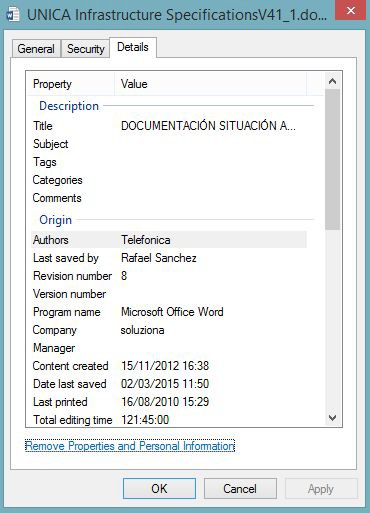
\includegraphics[width=\textwidth,height=0.8\textheight,keepaspectratio]{img/sl043.jpg}
\end{center}
\end{column}
\end{columns}
\end{frame}

\begin{frame}{Metadatos}
\footnotesize
\begin{columns}[c]
\begin{column}{0.55\textwidth}
  \begin{itemize}
  \item El comando strings en Unix también nos da información sobre las ``cadenas'' de texto que hay en el fichero
  \item Los metadatos en imágenes (jpeg) nos revelan información del contexto en el que se hizo la foto:
    \begin{itemize}
    \item Cámara
    \item Distancia focal, etc
    \item Geolocalización de la foto
    \end{itemize}
  \end{itemize}
\end{column}
\begin{column}{0.43\textwidth}
\begin{center}
\includegraphics[width=\textwidth,height=0.8\textheight,keepaspectratio]{img/sl044.jpg}
\end{center}
\end{column}
\end{columns}
\end{frame}

\begin{frame}{Herramientas generales para metadatos:}
\footnotesize
\begin{columns}[c]
\begin{column}{0.72\textwidth}
  \begin{itemize}
  \item \href{https://exiftool.org/}{Exiftool}
    \begin{itemize}
    \item \href{https://tools.kali.org/information-gathering/metagoofil}{Metagoofil}
    \item \href{https://www.elevenpaths.com/es/innovacion-laboratorio/herramientas/foca}{FOCA} (\href{https://www.elladodelmal.com/2009/04/foca-manual-de-usuario-i-de-iv.html}{Documentación})
    \item \href{https://www.maltego.com/}{Maltego}
    \item \href{https://metashieldclean-up.elevenpaths.com/}{Metashield Analyzer}
    \item \href{https://github.com/x0rz/tweets_analyzer}{Tweets Analyzer}
    \end{itemize}
  \item Ejemplos:
    \begin{itemize}
    \item \href{https://fwhibbit.es/pentesting-con-metadatos}{Caso de Uso 1}
    \item Caso de Uso 2: \href{https://youtu.be/xGeDkZxcBmw}{parte1}, \href{https://www.youtube.com/watch?v=QfYfvuPbd7Y}{parte2}
    \item Caso de Uso 3: \href{https://www.youtube.com/watch?v=y9gTqW5HB8Q}{parte1}, \href{https://www.youtube.com/watch?v=IDgfhAOR4nc}{parte2}
    \end{itemize}
  \end{itemize}
\end{column}
\begin{column}{0.26\textwidth}
\begin{center}
\includegraphics[width=\textwidth,height=0.55\textheight,keepaspectratio]{img/sl054.png}
\end{center}
\end{column}
\end{columns}
\end{frame}

\begin{frame}[allowframebreaks]{Metadatos}
\small
  \begin{itemize}
  \item Búsqueda inversa de imágenes: Lo de ``inversa'' se le añade para dejar claro que con este método no se buscan imágenes a partir de una palabra clave (lo que pones en el buscador), sino que se utiliza una imagen para obtener información derivada.
  \item Herramientas: \href{https://tineye.com/}{TinEye}
  \item También existen aplicaciones para crear imágenes artificiales, para usar, por ejemplo, como foto de un posible perfil falso
  \item Herramientas: \href{https://rosebud.ai/}{Rosebud AI}
  \item Y herramientas para determinar si una imagen ha sido modificada (muy útil para el ámbito forense): \href{https://fotoforensics.com/}{FotoForensics}
  \item Herramienta para posicionar vía metadatos la ubicación de las fotos: \href{https://www.pic2map.com/}{pic2map}
  \end{itemize}
\end{frame}

\begin{frame}[allowframebreaks]{Metadatos}
  \small
Metadatos y google hacking:
\begin{center}
\includegraphics[width=0.72\textwidth,height=0.58\textheight,keepaspectratio]{img/sl053.png}
\end{center}
\end{frame}

\begin{frame}{Ejercicio}
\small
\begin{center}
\includegraphics[width=0.45\textwidth,height=0.4\textheight,keepaspectratio]{img/sl057.jpg}
\end{center}
\vspace{0.5em}
  \begin{itemize}
  \item Usando google, localiza un fichero (doc, jpeg) de la organización a estudio y realiza un estudio de sus metadatos
  \end{itemize}
\end{frame}

\begin{frame}[allowframebreaks]{Metadatos}
\small
\href{pimeyes.com/es}{PimEyes}: Búsqueda Inversa de Rostros
  \begin{itemize}
  \item PimEyes es un motor de búsqueda inversa de imágenes especializado en rostros. A diferencia de Google Images o TinEye, está optimizado para identificar personas.
  \item Casos de uso en OSINT:
   \begin{itemize}
  \item Identificar si una persona usa la misma foto de perfil en distintas plataformas
  \item Localizar perfiles en redes sociales a partir de una única foto
  \item Verificar si una imagen de perfil es real o generada por IA (thispersondoesnotexist)
  \item Descubrir cuentas alternativas (sockpuppets) usadas por el mismo individuo
    \end{itemize}

  \item Funcionamiento:

    \begin{itemize}

  \item Sube una foto $\rightarrow$ PimEyes busca en millones de páginas web y RRSS
  \item Devuelve URLs donde aparece el mismo rostro con puntuación de similitud
  \item $\rightarrow$ Muy potente para perfilar individuos en investigaciones OSINT avanzadas
  \item $\rightarrow$ Combinado con Sherlock o Holehe permite un perfil completo de identidad digital
    \end{itemize}

  \end{itemize}
\end{frame}



\begin{frame}{Metadatos}
\footnotesize
\begin{columns}[c]
\begin{column}{0.55\textwidth}
  \begin{itemize}
  \item Los metadatos / cabeceras de los correos electrónicos (emails) también revelan información sensible e útil para un ataque
  \item Herramientas:
  \item \href{https://mxtoolbox.com/EmailHeaders.aspx}{MxToolbox} (Email Header Analyzer)
  \end{itemize}
\end{column}
\begin{column}{0.43\textwidth}
\begin{center}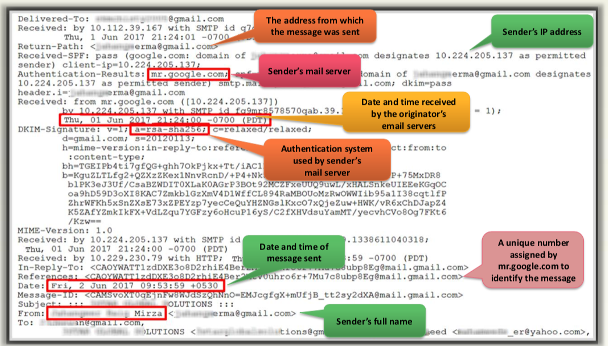
\includegraphics[width=\textwidth,height=0.8\textheight,keepaspectratio]{img/sl045.png}
\end{center}
\end{column}
\end{columns}
\end{frame}




\begin{frame}{Ejercicio}
\small
\begin{center}
\includegraphics[width=0.45\textwidth,height=0.4\textheight,keepaspectratio]{img/sl046.jpg}
\end{center}
\vspace{0.5em}
  \begin{itemize}
  \item Usa la opción de ``ver original'' de un correo en Gmail para ver los metadatos de un correo y, usa la herramienta Mxtoolbox para extraerlos
  \item ¿Qué es SPF y DKIM?
  \end{itemize}
\end{frame}

\begin{frame}[allowframebreaks]{Ejercicio}
\small
  \begin{itemize}
  \item \href{https://tryhackme.com/room/ohsint}{Realiza esta room en tryhackme sobre OSINT: ohSint}
  \end{itemize}
\begin{center}
\includegraphics[width=0.72\textwidth,height=0.58\textheight,keepaspectratio]{img/sl047.jpg}
\end{center}
\end{frame}

\section{Seguridad del correo electrónico}

\begin{frame}[allowframebreaks]{Seguridad en el correo electrónico}
\small
SPF (Sender Policy Framework):
  \begin{itemize}
  \item Es una protección contra la falsificación de direcciones en el envío de correo electrónico.
  \item Identifica, a través de los registros de nombres de dominio (DNS) --registro MX-, a los servidores de correo SMTP autorizados para el transporte de los mensajes.
  \item SPF extiende el protocolo SMTP para permitir comprobar las máquinas autorizadas a enviar correo para un dominio determinado. La idea esidentificar las máquinas autorizadas por su dirección IP, y que esta identificación la haga el responsable del dominio que recibirá el correo.
  \item Previene frente a spam y phishing
  \item Cómo se configura:
  \item midominio.com. IN TXT \textquotedbl{}v=spf1 mx ptr \textasciitilde{}all\textquotedbl{}
  \end{itemize}
\end{frame}

\begin{frame}{Seguridad en el correo electrónico}
\footnotesize
DKIM (Domain Keys Identified Mail):
  \begin{itemize}
  \item Es un mecanismo de autenticación de correo electrónico que permite a una organización responsabilizarse del envío de un mensaje, de manera que éste pueda ser validado por un destinatario.
  \item DKIM utiliza criptografía de clave pública para permitir al origen firmar electrónicamente correos electrónicos legítimos de manera que puedan ser verificados por los destinatarios. Cualquier correo originado desde estas organizaciones deben llevar una firma (cabeceras y cuerpo) DKIM.
  \item En la mayoría de los casos el módulo firmante actúa en nombre de la organización originaria insertando una firma DKIM en las cabeceras del mensaje, y el módulo de comprobación en nombre de la organización del receptor, validando la firma obteniendo la clave pública del firmante a través del DNS
  \item El servidor SMTP utiliza el nombre de dominio perteneciente al emisor, la cadena \textquotedbl{}\_domainkey\textquotedbl{}, y un selector del campo de la firma DKIM para realizar una consulta al DNS. La respuesta debe incluir la clave pública del dominio.
  \end{itemize}
\end{frame}

\begin{frame}{Seguridad en el correo electrónico}
\footnotesize
DMARC --- Protección contra suplantación de correo:
  \begin{itemize}
  \item DMARC (Domain-based Message Authentication, Reporting \& Conformance) es un protocolo de autenticación de correo electrónico que ayuda a prevenir el spoofing y el phishing usando dominios falsos.
  \item Se basa en dos mecanismos existentes:
    \begin{itemize}
  \item SPF (Sender Policy Framework)
  \item DKIM (DomainKeys Identified Mail)
    \end{itemize}
  \item El propietario del dominio publica en su DNS una política DMARC que indica qué hacer con los correos que fallen las verificaciones (aceptar, poner en cuarentena o rechazar)
  \item Dónde enviar los reportes de fallos o intentos de suplantación
  \item \href{https://mxtoolbox.com/dmarc.aspx}{DMARC checker}
  \item \href{https://www.linkedin.com/posts/thomasoneil\%C3\%A1lvarez_ciberseguridad-emailsecurity-ethicalhacking-activity-7300978336397213696-Kn7E/}{SpoofThatMail} --- comprueba si un dominio se puede suplantar (SPF/DMARC ausentes o débiles)
  \end{itemize}
\vfill
\begin{center}
\includegraphics[width=0.60\textwidth,height=0.24\textheight,keepaspectratio]{img/sl050.png}
\end{center}
\end{frame}


\begin{frame}{Seguridad en el correo electrónico}
\begin{center}
\includegraphics[width=\textwidth,height=0.82\textheight,keepaspectratio]{img/sl051.png}\end{center}
\end{frame}

\begin{frame}{Seguridad en el correo electrónico}
\begin{center}
\includegraphics[width=\textwidth,height=0.82\textheight,keepaspectratio]{img/sl052.png}\end{center}
\end{frame}

\begin{frame}[allowframebreaks]{Seguridad en el correo electrónico}
\small
Estos protocolos protegen el correo, pero su \textbf{ausencia} es un vector de ataque clave:
  \begin{itemize}
  \item \textbf{Sin DMARC: email spoofing directo}
    \begin{itemize}
    \item El atacante envía un email como \cmd{ceo@empresa-real.com} desde su propio servidor.
    \item Si DMARC tiene política \cmd{p=none} (solo monitorización), el correo llega igualmente.
    \item $\rightarrow$ Base de ataques BEC (Business Email Compromise), con fraudes de millones de euros.
    \end{itemize}
  \item \textbf{Comprobación rápida en footprinting}
    \begin{itemize}
    \item \cmd{dig TXT empresa.com} $\rightarrow$ ver registro SPF
    \item \cmd{dig TXT \_dmarc.empresa.com} $\rightarrow$ ver política DMARC
    \item Si devuelve \cmd{p=none} o no hay registro $\rightarrow$ dominio vulnerable a spoofing.
    \end{itemize}
  \item \textbf{Herramientas}
    \begin{itemize}
    \item \href{https://mxtoolbox.com}{mxtoolbox.com} $\cdot$ \href{https://dmarcian.com}{dmarcian.com} $\cdot$ \href{https://github.com/a6avind/spoofcheck}{spoofcheck}
    \item $\rightarrow$ Un dominio sin DMARC estricto permite suplantar a cualquier empleado por email.
    \end{itemize}
  \end{itemize}
\end{frame}

\section{whois \& alertas}

\begin{frame}{whois \& alertas}
\small
\begin{columns}[c]
\begin{column}{0.68\textwidth}
  \begin{itemize}
  \item La base de datos whois es mantenida por Regional Internet Registries y contiene información personal sobre los propietarios de los dominios. En una consulta se puede obtener información como:
    \begin{itemize}

  \item Nombre del contacto / administrador
  \item Servidores DNS
  \item Rango de red
  \item Cuando se creó el dominio y cuando expira
  \item Última actualización
  \item Herramienta: \href{https://www.whois.com/whois/}{Whois.com} $\cdot$ \href{https://lookup.icann.org/}{ICANN Lookup}
  \end{itemize}
    \end{itemize}
\end{column}
\begin{column}{0.30\textwidth}
\begin{center}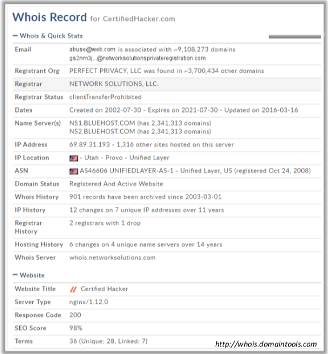
\includegraphics[width=\textwidth,height=0.7\textheight,keepaspectratio]{img/sl058.png}
\end{center}
\end{column}
\end{columns}
\end{frame}

\begin{frame}{whois \& alertas}
\footnotesize
  \begin{itemize}
  \item Son avisos que se pueden programar para notificar al auditor cuando se produce algún cambio en los activos (dominios, RRSS, etc) de la organización objetivo
  \item Herramientas:
    \begin{itemize}
    \item \href{https://www.google.com/alerts}{Google Alerts}
    \item \href{https://pro.x.com/}{X Pro} (antes TweetDeck): columnas de seguimiento en X/Twitter
    \item \href{https://archive.org/}{Archive.org}
      \begin{itemize}
      \item Es una web en la que se almacenan el histórico de los contenidos de dominios y se pueden consultar.
      \end{itemize}
    \end{itemize}
  \end{itemize}
\vfill
  \begin{center}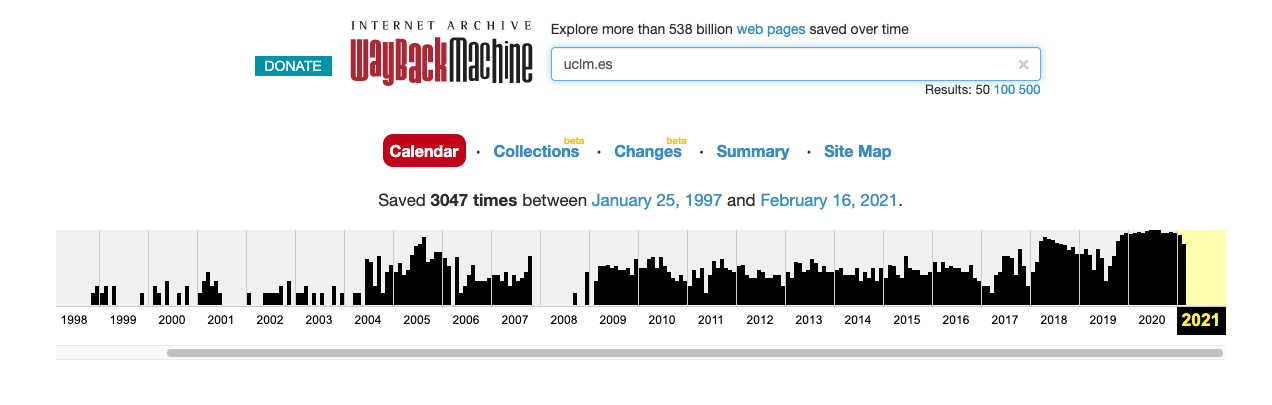
\includegraphics[width=0.85\textwidth,height=0.38\textheight,keepaspectratio]{img/sl059.png}
\end{center}
\end{frame}

\begin{frame}[allowframebreaks]{whois \& alertas}
\small
Caché google: Similar a archive.org
\begin{center}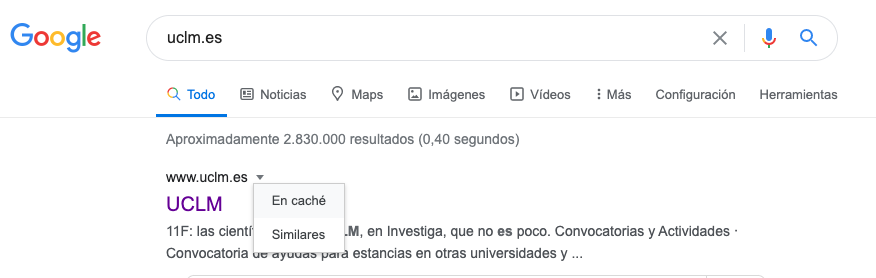
\includegraphics[width=0.72\textwidth,height=0.58\textheight,keepaspectratio]{img/sl060.png}
\end{center}
\end{frame}

\section{Metodología para averiguar infraestructura}

\begin{frame}{Metodología para averiguar infraestructura}
\small
  \begin{itemize}
  \item El proceso de obtención de información inicial en ejercicios amplios como Red Team consiste en ser capaz de identificar la infraestructura completa dentro del alcance, para lo cual es recomendable seguir el siguiente enfoque:
  \end{itemize}
\vfill
\begin{center}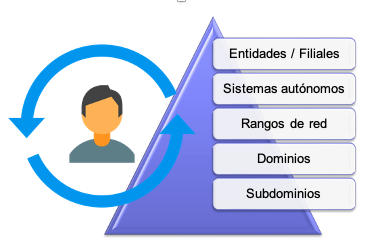
\includegraphics[width=0.55\textwidth,height=0.6\textheight,keepaspectratio]{img/sl062.png}
\end{center}
\end{frame}

\begin{frame}{Metodología para averiguar infraestructura}
\small
Análisis general de la organización
\begin{columns}[c]
\begin{column}{0.72\textwidth}
  \begin{itemize}
  \item Para comenzar el proceso de forma correcta por lo tanto, será necesario conocer bien la organización, y cuales son las entidades dentro del alcance. Para ello será necesario realizar búsquedas para obtener:
    \begin{itemize}
  \item Identificación de nombres anteriores
  \item Identificación de nombres diferentes en otros países
  \item Identificación de filiales o empresas de las que es propietaria
  \item Identificación de proveedores
  \item Para ello se puede hacer uso de aplicaciones de noticias, Wikipedia, \dots{}
  \end{itemize}
  \end{itemize}
\end{column}
\begin{column}{0.26\textwidth}
\begin{center}
\includegraphics[width=\textwidth,height=0.55\textheight,keepaspectratio]{img/sl063.jpg}
\end{center}
\end{column}
\end{columns}
\end{frame}

\begin{frame}[allowframebreaks]{Metodología para averiguar infraestructura}
\small
Identificación de sistemas autónomos
  \begin{itemize}
  \item Una vez se conocen las entidades dentro del alcance es necesario identificar los sistemas autónomos para cada una de dichas entidades. Esto puede ser realizado mediante múltiples servicios online tales como:
    \begin{itemize}
  \item \href{http://ipv4info.com/}{ipv4info.com}
  \item \href{https://bgp.he.net/}{bgp.he.net} (Hurricane Electric BGP Toolkit)
  \item \href{https://www.robtex.com/}{robtex.com}
    \end{itemize}

  \item Herramienta: \href{https://bgp.he.net/}{ASN Lookup Tool and Traceroute Server}
      \begin{itemize}
  \item Permitirá obtener gran cantidad de rangos de red, aunque muy probablemente no todos lo que se encuentran dentro del alcance de las pruebas. Sirve como punto de partida, al que posteriormente retornar para volver a realizar otra iteración.
  \item Las direcciones IPs en internet se reparten o se asocian a sistemas autónomos, que no es más que un bloque de Ips. El protocolo BGP realiza encaminamiento entre sistemas autonomos
      \end{itemize}

  \item También existe la opción de descargar esta información de fuentes como:
      \begin{itemize}
  \item ARIN: \href{https://ftp.arin.net/info/asn.txt}{ftp.arin.net/info/asn.txt}
  \item APNIC: \href{https://ftp.apnic.net/transfers/apnic/transfer-apnic-latest}{transfer-apnic-latest}
       \end{itemize}

  \item O directamente consultarla a los RIRs mediante WHOIS, tal y como se muestra en las siguientes consultas:
       \begin{itemize}
  \item whois -h whois.arin.net \textquotedbl{}a 701``
  \item whois -h whois.arin.net \textquotedbl{}a 701\textquotedbl{} | grep -Eo \textquotedbl{}([0--9.]+)\{4\}/[0--9]+\textquotedbl{}
  \item Esto permite la automatización de acciones.
       \end{itemize}

\end{itemize}
\end{frame}

\begin{frame}{Metodología para averiguar infraestructura}
\footnotesize
\begin{columns}[c]
\begin{column}{0.62\textwidth}
  \begin{itemize}
  \item Este mismo proceso podría ser utilizado adicionalmente para obtener más información tales hacer búsquedas inversas que permitan identificar información adicional como correos de la compañía objetivo que han sido utilizados para registrar activos, y buscar posteriormente dichos activos.
  \item Más filtros:
  \begin{itemize}
  \item \href{https://www.arin.net/resources/registry/whois/rws/cli/}{ARIN Whois-RWS (CLI)}
    \end{itemize}
  \item Existen ataques a sistemas autónomos / protocolo BGP:
    \begin{itemize}
    \item \href{https://manrs.org/2020/09/what-is-bgp-prefix-hijacking-part-1/}{MANRS --- What is BGP prefix hijacking?}
    \item \href{https://www.kentik.com/kentipedia/bgp-hijacking/}{Kentik --- BGP Hijacking: threats to Internet routing}
    \end{itemize}
  \item Al igual que el caso mostrado anteriormente, la mayoría de RIRs (Regional Internet Registries) también permiten hacer búsquedas muy centradas en un objetivo a través de su servicio, como en el caso de \href{https://apps.db.ripe.net/db-web-ui/query}{RIPE}

  \end{itemize}
\end{column}
\begin{column}{0.36\textwidth}
\begin{center}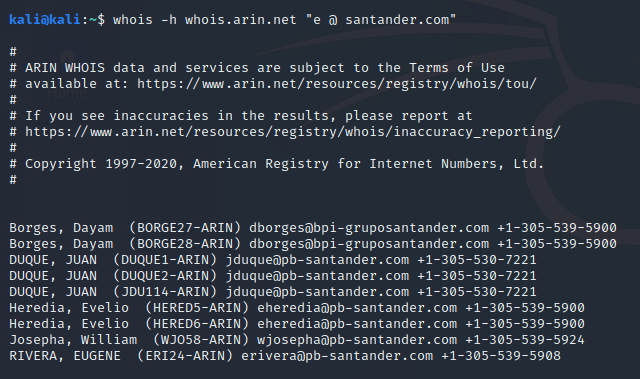
\includegraphics[width=\textwidth,height=0.75\textheight,keepaspectratio]{img/sl065.png}
\end{center}
\end{column}
\end{columns}
\end{frame}


\begin{frame}[allowframebreaks]{Metodología para averiguar infraestructura}
\small
Identificación de rangos de red
  \begin{itemize}
  \item Conocer todos los rangos de red que están dentro del alcance es un aspecto crítico, pues en última instancia, permite posteriormente desarrollar los escaneos de red necesarios para identificar cuales de estos sistemas están vivos y cuales son los servicios habilitados que tienen. Al igual que en el caso anterior, se puede hacer búsquedas en aplicaciones como IPv4info mediante campos de red:
  \end{itemize}
\begin{center}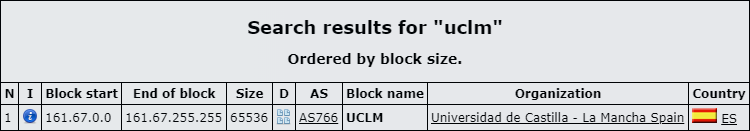
\includegraphics[width=0.72\textwidth,height=0.58\textheight,keepaspectratio]{img/sl067.png}
\end{center}
\end{frame}

\begin{frame}{Ejercicio}
\small
\begin{center}
\includegraphics[width=0.45\textwidth,height=0.4\textheight,keepaspectratio]{img/sl068.jpg}
\end{center}
\vspace{0.5em}
  \begin{itemize}
  \item Identifica el sistema autónomo y los rangos de red asociados a la organización bajo estudio
  \end{itemize}
\end{frame}

\begin{frame}[allowframebreaks]{Metodología para averiguar infraestructura}
\small
Identificación de dominios
  \begin{itemize}
  \item Una vez se conoce la infraestructura de red pública es necesario pasar a la identificación de los dominios principales, pues hoy en día las aplicaciones web son, en muchos casos, la forma de acceder a la red interna de una entidad. Algunas de las acciones que pueden ser realizadas para ello son:
  \begin{itemize}
  \item Identificación mediante la resolución inversa de direcciones IP
  \item Identificación mediante compartición de NS y MX (\href{https://viewdns.info}{ViewDNS})
  \item Identificación mediante Google Hacking (u otros buscadores)
  \end{itemize}
  \item Es importante remarcar que antes de buscar subdominios es recomendable buscar bien los dominios principales. Si bien, todos los dominios y subdominios deberán ser correctamente registrados.
  \end{itemize}
\end{frame}

\begin{frame}[allowframebreaks]{Metodología para averiguar infraestructura}
\small
  \begin{itemize}
  \item En caso de haber hecho uso de IPv4info o servicios similares, además de identificar rangos de red será posible obtener una primera aproximación de dominios y subdominios existentes que permitirá posteriormente profundizar.
  \item Uno de los ejemplos previos expuestos que puede permitir la identificación de dominios y subdominios es la comprobación de servidores MX o NS compartidos, con servicios como ViewDNS

  \end{itemize}
\end{frame}


\begin{frame}[allowframebreaks]{Metodología para averiguar infraestructura}
\small
Identificación de subdominios
  \begin{itemize}
  \item Una vez identificados los dominios principales, es momento de pasar a identificar el mayor número de subdominios posibles para cada dominios principal identificado. Para ello se puede optar por múltiples opciones como:
    \begin{itemize}
  \item Servicios públicos: \href{https://securitytrails.com/}{SecurityTrails} (antes FindSubdomains)
  \item Resolución inversa de direcciones IP: \href{https://viewdns.info/}{ViewDNS}
  \item Google Hacking (u otros buscadores)
  \item Búsqueda en registros de \textbf{Certificate Transparency} (CT logs): \href{https://crt.sh}{crt.sh} o \href{https://search.censys.io/}{Censys}
   \begin{itemize}
  \item muchas empresas usan el mismo certificado para varios subdominios..observando éstos podemos identificarlos.
   \end{itemize}
  \item Otras posibilidades: \href{https://dnsdumpster.com/}{DNSdumpster}, \href{https://transparencyreport.google.com/https/certificates}{Google Transparency Report}, \href{https://www.virustotal.com/}{VirusTotal}, \dots{}
  \item también con ataques de transferencia a de zona (se verán más adelante)
  \item Fuerza bruta (activa): \href{https://github.com/eredotpkfr/subscan}{subscan}, \href{https://github.com/blechschmidt/massdns}{massdns}, \href{https://github.com/infosec-au/altdns}{altdns}, \dots{}
  \item A partir de los Certificate Transparency Logs: herramienta \href{https://github.com/UnaPibaGeek/ctfr}{CTFR}

  \end{itemize}

\end{itemize}
\end{frame}

\begin{frame}[allowframebreaks]{Metodología para averiguar infraestructura}
\small
Herramientas que pueden automatizar el proceso como:
  \begin{itemize}
  \item \href{https://github.com/aboul3la/Sublist3r}{Sublist3r}
    \item \href{https://github.com/projectdiscovery/subfinder}{subfinder}
    \item \href{https://github.com/owasp-amass/amass}{Amass}
    \item \href{https://github.com/michenriksen/aquatone}{Aquatone}
    \item \href{https://github.com/tomnomnom/assetfinder}{assetfinder} $\cdot$ \href{https://github.com/findomain/findomain}{findomain}
    \item \href{https://github.com/projectdiscovery/dnsx}{dnsx} --- resolución masiva y filtrado de subdominios \emph{vivos}
    \item (se verán en detalle en la unidad de enumeración)
    \item (matiz: hay herramientas para enumerar dominios y otras para hacer OSINT de dominios)
  \item Ejemplo: \href{https://fwhibbit.es/wh01p-que-hay-detras-de-esa-ip}{leer}
  \end{itemize}
\end{frame}

\begin{frame}[allowframebreaks]{Metodología para averiguar infraestructura}
\small
  \begin{itemize}
  \item De todas las opciones previas, \href{https://github.com/owasp-amass/amass}{Amass}, es sin duda uno de los frameworks más potentes actualmente que se encuentra en constante desarrollo por OWASP. Se muestran a continuación algunos ejemplos de las capacidades destacadas:
  \begin{itemize}

  \item Búsqueda en fuentes abiertas para la identificación sin información previa
  \item Distinción entre enumeración pasiva y activa
  \item Proporción de las fuentes utilizadas
  \item Generación y mapeo de activos en gráficos
    \end{itemize}
  
  \item Opciones completas: \href{https://github.com/owasp-amass/amass/blob/master/doc/tutorial.md}{Tutorial de Amass} $\cdot$ \href{https://owasp.org/www-project-amass/}{Proyecto OWASP Amass}
  \item Ejemplos de uso:
    \begin{itemize}

    \item Identificación de dominios con características similares en WHOIS: amass intel -d fraternidad.com -whois
  \item Identificación de subdominios, mostrando la fuente: amass enum -d fraternidad.com -src
  \item Identificación de subdominios de forma pasiva, mostrando la fuente: amass enum -passive -d fraternidad.com -src
  \end{itemize}
  \end{itemize}

\end{frame}


\begin{frame}[allowframebreaks]{Metodología para averiguar infraestructura}
\small
  \begin{itemize}
  \item Además de hacer uso de herramientas completas como Amass, también es recomendable hacer búsquedas dirigidas por servicio, como por ejemplo CRT.sh, que puede permitir la identificación de posibles dominios y subdominios en preproducción.
  \item Ejemplo de búsquedas en crt.sh:
    \begin{itemize}

  \item \%.uclm.es
    \end{itemize}

  \item Una vez conocida una IP/dominio, se puede determinar si ésta esta comprometida (threat hunting).
  \item Herramientas:
      \begin{itemize}

  \item \href{https://github.com/ninoseki/mihari}{mihari}
  \end{itemize}
  

  \end{itemize}
\end{frame}

\begin{frame}{Ejercicio}
\small
\begin{center}
\includegraphics[width=0.45\textwidth,height=0.4\textheight,keepaspectratio]{img/sl077.jpg}
\end{center}
\vspace{0.5em}
  \begin{itemize}
  \item Utiliza la herramienta sublist3er/amass (o similares) para encontrar dominios y sub-dominios de la organización a estudio.
  \end{itemize}
\end{frame}

\section{Footprinting web}

\begin{frame}[allowframebreaks]{Footprinting web}
\small
  \begin{itemize}
  \item Esta técnica consiste en monitorizar y analizar las webs encontradas en el ejercicio anterior. La información que se puede recopilar:
  \begin{itemize}

  \item Software y versión
  \item Sistema operativo y lenguajes (servidor, scripting)
  \item Nombre de ficheros, rutas, bases de datos, consultas a las bases de datos
  \item Detalles de contacto
  \item CMS usando
  \end{itemize}
  \item Herramientas:
  \begin{itemize}
  \item Proxies webs: Burp Suite, ZAP
  \item Banner grabbing
  \end{itemize} 
  \end{itemize}
\end{frame}

\begin{frame}{Footprinting web}
\footnotesize
Examinar el código fuente (html); puedes encontrar:
  \begin{itemize}
  \item Comentarios del desarrollador
    \begin{itemize}
    \item Detalles de contacto del administrador o desarrollador
    \item Estructura del sistema de ficheros
    \item Tecnologías de scripting o de la base de datos
    \end{itemize}
  \item Examinar las cookies:
    \begin{itemize}
    \item Software usado (ejemplo, c1.Microsoft.com)
    \item Lenguaje de scripting
    \end{itemize}
  \end{itemize}
\vfill
\begin{center}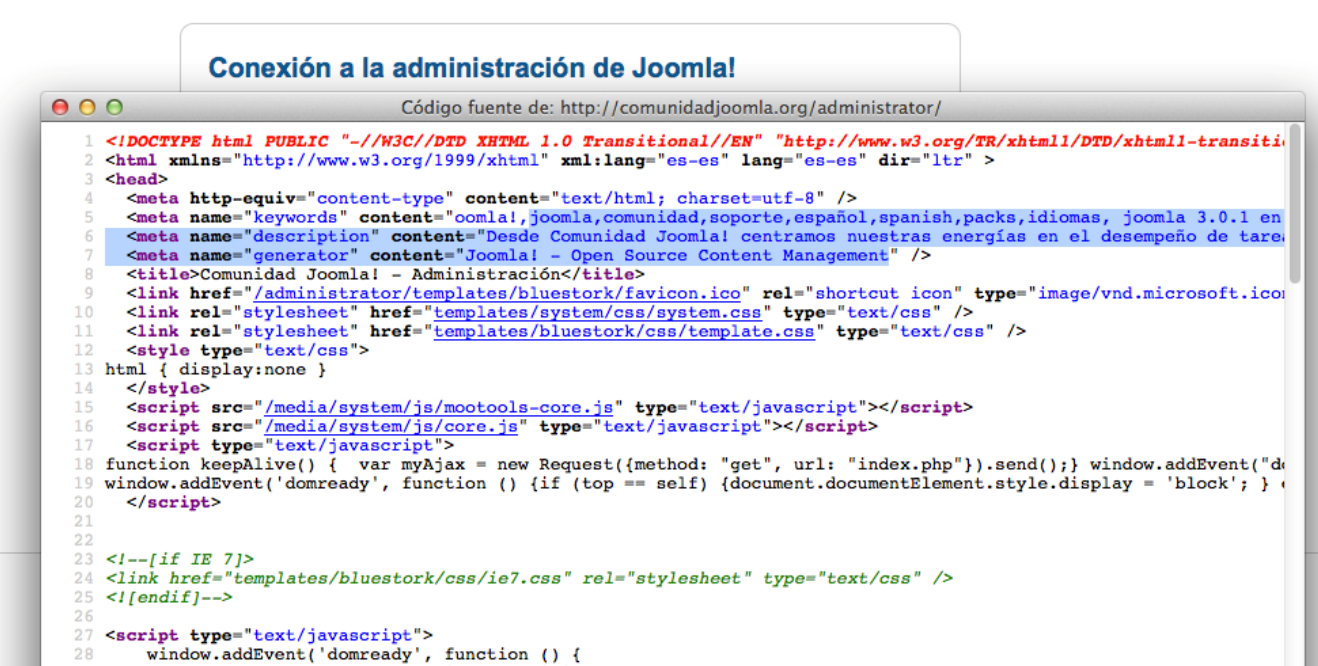
\includegraphics[width=0.8\textwidth,height=0.42\textheight,keepaspectratio]{img/sl079.png}
\end{center}
\end{frame}

\begin{frame}[allowframebreaks]{Footprinting web}
\small
Web spider:
  \begin{itemize}
  \item Realizan búsquedas de manera automática (y recursiva) por la web
  \item Herramientas
  \begin{itemize}
  \item \href{https://github.com/smicallef/spiderfoot}{Spiderfoot} (\href{https://www.osintux.org/documentacion/spiderfoot}{documentación})
    \end{itemize}
  \item Mirroring website: Consiste en hacer una copia exacta del dominio y subdominios en una estructura de ficheros local, incluyendo ficheros html, pdfs, imágenes, etc
  \item Herramientas:
  \begin{itemize}
  \item \href{https://github.com/httparchive/httrack}{Httrack}
  \end{itemize}
\end{itemize}
\end{frame}

\begin{frame}[allowframebreaks]{Footprinting web}
\small
Mensajes de error
  \begin{itemize}
  \item Si solicitamos una url que no existe, el servidor web nos devuelve un error 404 y, si no está bien configurado las respuestas de error, muestra información sensible, por ejemplo:
  \end{itemize}
\begin{center}
\includegraphics[width=0.72\textwidth,height=0.58\textheight,keepaspectratio]{img/sl081.png}
\end{center}
\end{frame}

\begin{frame}[allowframebreaks]{Footprinting web}
\small
Banner grabbing
  \begin{itemize}
  \item Interactuando ``en crudo'' con el servidor web, podemos ver las respuestas de éste y, en ella podemos ver información sensible
  \end{itemize}
\begin{center}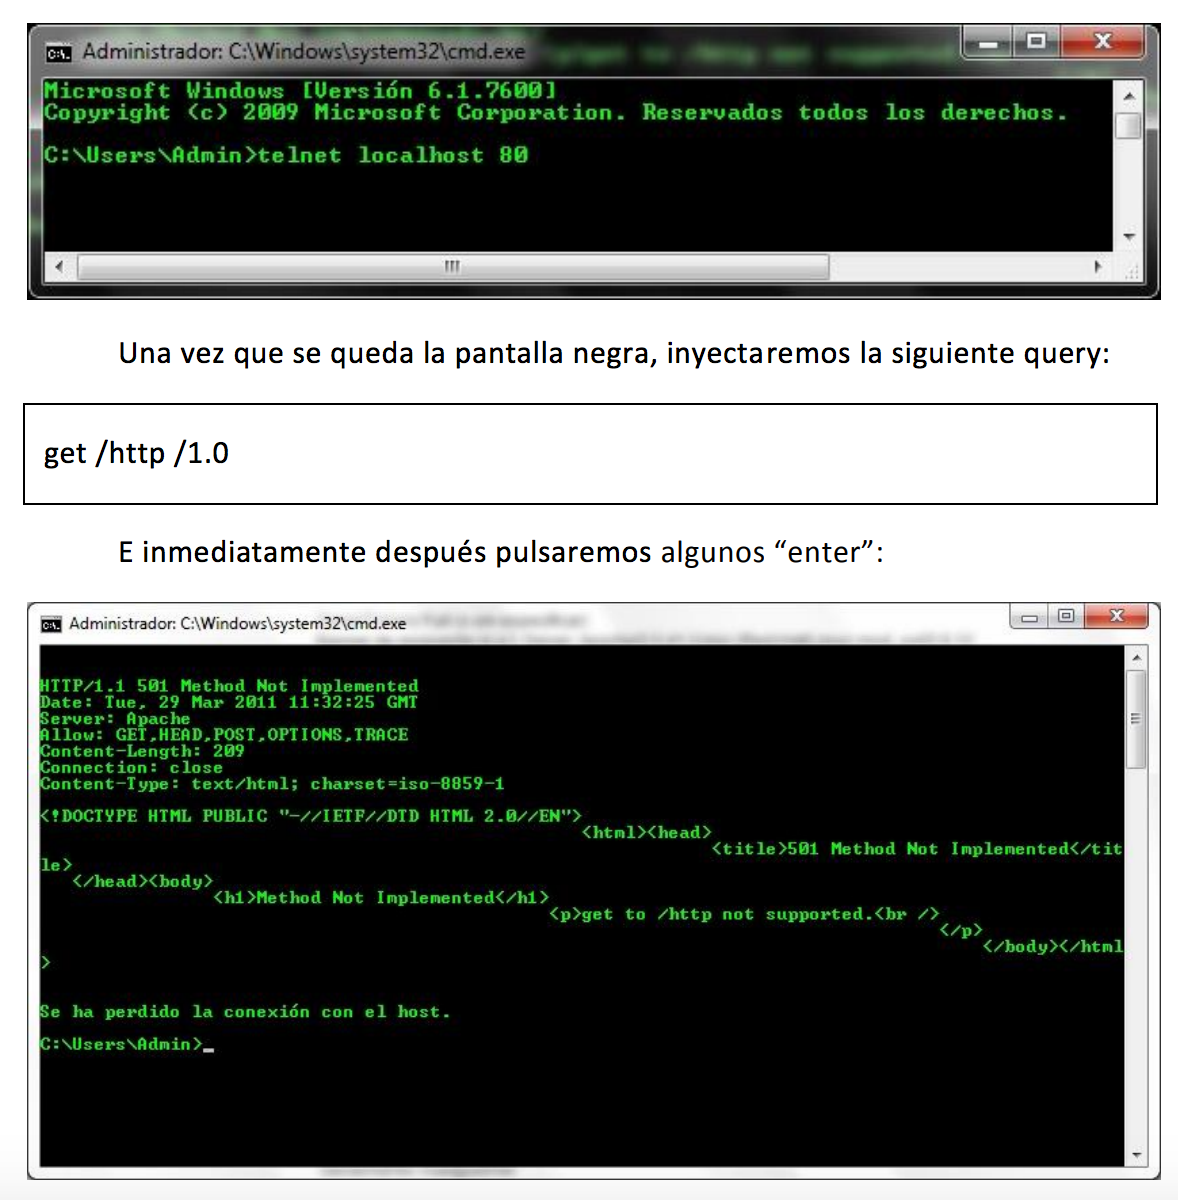
\includegraphics[width=0.72\textwidth,height=0.58\textheight,keepaspectratio]{img/sl082.png}
\end{center}
\end{frame}

\begin{frame}{Footprinting web}
\small
Robots.txt
  \begin{itemize}
  \item ¿Qué páginas no queremos que busquen?
  \item Un archivo robots.txt es un archivo que se encuentra en la raíz de un sitio e indica a qué partes no quieres que accedan los crawlers o rastreadores de los motores de búsqueda.
  \item Un crawler es un robot de una entidad (generalmente buscadores) que acceden a las páginas web de un sitio para buscar información en ella, añadirla en los buscadores, etc.
  \end{itemize}
\vfill
\begin{center}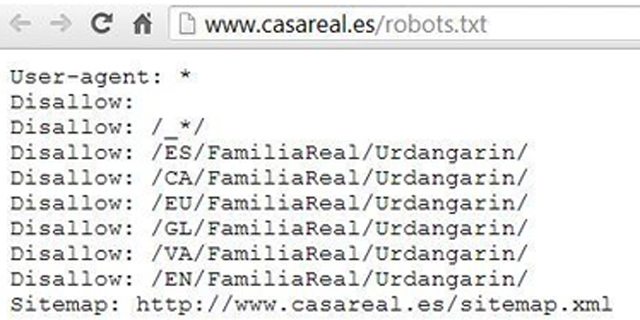
\includegraphics[width=0.62\textwidth,height=0.45\textheight,keepaspectratio]{img/sl083.jpg}
\end{center}
\end{frame}

\begin{frame}[allowframebreaks]{Footprinting web}
\small
Herramientas todo en uno para footprinting web (url):
  \begin{itemize}
  \item \href{https://hakin9.org/final-recon-osint-tool-for-all-in-one-web-reconnaissance/}{final-recon}
  \item \href{https://urlscan.io/}{urlscan.io}
  \end{itemize}
\end{frame}

\begin{frame}{Ejercicio}
\small
\begin{center}
\includegraphics[width=0.45\textwidth,height=0.4\textheight,keepaspectratio]{img/sl085.jpg}
\end{center}
\vspace{0.5em}
  \begin{itemize}
  \item A partir de alguna de las urls encontradas, comprueba si los mensaje de error dan información sensible, si el robots.txt esconde algunos dominios no accesible via google, comprueba el código fuente de la página y realiza técnicas de banner grabbing para recopilar información sensible
  \end{itemize}
\end{frame}

\section{Geolocalización IP}

\begin{frame}[allowframebreaks]{Geolocalización IP}
\small
  \begin{itemize}
  \item Geolocalización de IP, nos puede dar información sobre el país, estado/región, ciudad, código postal, uso horario, velocidad de conexión, proveedor de servicio (ISP)
  \item Herramienta:
    \begin{itemize}

  \item Geo-rcon
  \item \href{https://www.iplocation.net/}{IP Location}
  \item \href{https://github.com/lksnyder0/geoip-lookup}{geoip-lookup}
  \item \href{https://github.com/maldevel/IPGeoLocation}{IPGeoLocation}
  \item \href{https://ipstack.com/}{ipstack}
  \item Coordenadas GPS
  \item \href{https://github.com/thewhiteh4t/seeker}{Seeker}
  \item \href{https://github.com/ilektrojohn/creepy}{Creepy}
    \end{itemize}
  \item \href{https://www.coordenadas-gps.com/}{Convertir de coordenadas GPS a ubicación}
  \end{itemize}
\end{frame}

\section{Virtual hosting}

\begin{frame}[allowframebreaks]{Virtual hosting:}
\small
  \begin{itemize}
    \item El virtual hosting es una técnica que permite a una sola máquina física o servidor web mostrar varios sitios web diferentes. 
    \item El servidor usa los nombres de los dominios o direcciones IP para enviar a cada usuario la página correcta.
    \item El servidor (Name-based): Usa una sola dirección IP para muchos sitios web distintos. El servidor lee el dominio que pides en el navegador y abre la página correcta. Es el método más común hoy en día.
    \item Ventajas principales:
      \begin{itemize}

    \item Ahorro de dinero: No necesitas comprar un ordenador o servidor físico para cada página web.
    \item Buen uso de recursos: Aprovecha al máximo la memoria y la fuerza del servidor principal.
    \item Fácil manejo: Ayuda a ordenar y controlar muchos proyectos desde un solo lugar       \end{itemize}

  \end{itemize}
\end{frame}

\begin{frame}{Virtual hosting:}
\footnotesize
\begin{columns}[c]
\begin{column}{0.76\textwidth}
      \begin{itemize}

  \item Determinar si varios dominios / urls están alojados en la misma IP usando host virtuales
    \item Herramientas:
      \begin{itemize}
      \item \href{https://github.com/dariusztytko/vhosts-sieve}{vhost-siege}
      \item \href{https://pentest-tools.com/information-gathering/find-virtual-hosts}{PentesterTool}
      \item Buscador bing (ip:161.67.137.16)
      \item \href{https://github.com/codingo/VHostScan}{VHostScan}
      \item NSE de nmap
      \item \href{https://search.censys.io/}{censys} y poner ip: dir ip
      \item \href{https://github.com/jobertabma/virtual-host-discovery}{virtual-host-Discovery}
      \item Recon-ng
    \end{itemize}
  \item Conocer si una IP a sido a un nodo TOR relay:
    \begin{itemize}
    \item \href{https://metrics.torproject.org/exonerator.html?s=03}{TORmetrics}
    \end{itemize}
    \end{itemize}
\end{column}
\begin{column}{0.22\textwidth}
\begin{center}
\includegraphics[width=\textwidth,height=0.5\textheight,keepaspectratio]{img/sl087.jpg}
\end{center}
\end{column}
\end{columns}
\end{frame}

\begin{frame}[allowframebreaks]{Virtual hosting:}
\small
\href{https://pentest-tools.com}{PentesterTools}

  \begin{center}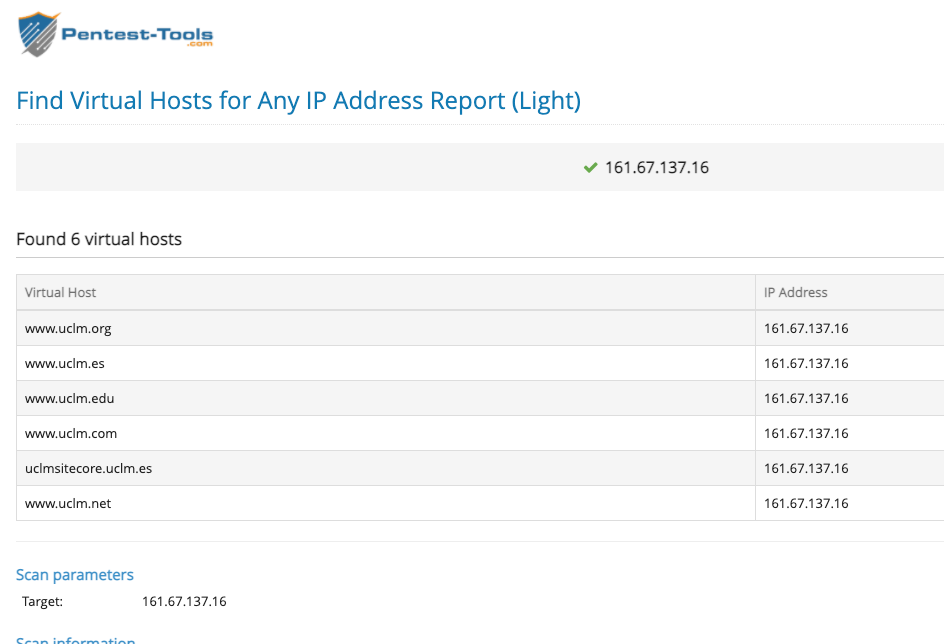
\includegraphics[width=0.72\textwidth,height=0.58\textheight,keepaspectratio]{img/sl086.png}
  \end{center}
\end{frame}

\section{Evasión de WAFs y balanceadores de carga}

\begin{frame}[allowframebreaks]{Evasión de WAFs y balanceadores de carga}
\small
  \begin{itemize}
  \item A veces ocurre que la IP que obtenemos es la IP de un WAF o un balanceador, como Cloudfare
  \item Estos servicios actúan como proxy y protegen la IP real, ofreciendo la IP del servicio.
  \item Protegen frente ataques DoS y también son útiles para balanceo de carga en caso de mucho tráfico
  \item Hay herramientas que guardan un histórico del DNS por si, en algún momento esas urls no hubieran estado detrás de un WAF y tener así, la IP real, por ejemplo:
  \item \href{https://github.com/Elsfa7-110/bypass-firewalls-by-DNS-history}{Bypass firewalls by abusing DNS history}
  \end{itemize}
\end{frame}

\begin{frame}[allowframebreaks]{Evasión de WAFs y balanceadores de carga}
\small
  \begin{itemize}
  \item Estos servicios ocultan la IP real del objetivo; existen herramientas para averiguar esa IP
    \begin{itemize}
    \item \href{https://github.com/jychp/cloudflare-bypass}{Cloudfare-bypass}
    \item \href{https://github.com/Warflop/CloudBunny}{Cloudbunny} (desactualizada)
    \item \href{https://github.com/EnableSecurity/wafw00f}{Wafw00f}
    \item \href{https://github.com/jmbr/halberd}{Halberd}
    \item \href{https://github.com/m0rtem/CloudFail}{cloudfail}
    \item Certificados SSL reutilizados: \href{https://censys.io/certificates?q=parsed.names\%3A+elhacker.net}{búsqueda en censys.io} (combinable con CloudFlair)
    \item Correo saliente (por ejemplo e-mail enviado registro blog, foro)
    \item Usando motores de búsqueda tipo Shodan
    \item Favicon Hash
    \item XML-RPC Pingback (en WordPress)
    \end{itemize}
  \item Conocer el proveedor de servicio a partir de una IP: \href{https://www.whoismyisp.org/}{whoismysip}
  \item \href{https://jychp.medium.com/how-to-bypass-cloudflare-bot-protection-1f2c6c0c36fb}{Lectura}
  \end{itemize}
\end{frame}

\begin{frame}[allowframebreaks]{Evasión de WAFs y balanceadores de carga}
\small
CloakQuest3r: IP Real detrás de Cloudflare
  \begin{itemize}
  \item CloakQuest3r es una herramienta específicamente diseñada para descubrir
  \item la IP de origen de servidores protegidos por Cloudflare u otros WAF/CDN.
  \item linkedin.com/posts/jemmie-orellana --- CloakQuest3r demo
  \item Técnicas que combina:
  \begin{itemize}
  \item Consulta de histórico DNS (SecurityTrails, ViewDNS) $\rightarrow$ IP antes del WAF
  \item Búsqueda en certificados SSL (crt.sh, Censys) con el mismo dominio
  \item Favicon hash matching en Shodan para localizar el servidor real
  \item Análisis de correos salientes (cabeceras SMTP revelan IP real del MTA)
  \item Búsqueda de subdominios sin protección WAF que apuntan a la IP real
  \end{itemize}
  \item Uso básico:
    \begin{itemize}

  \item pip install cloakquest3r
  \item cloakquest3r -d empresa.com
  \end{itemize}

\end{itemize}
\end{frame}

\begin{frame}[allowframebreaks]{Evasión de WAFs y balanceadores de carga}
\small
  \begin{itemize}
  \item La herramienta \href{https://github.com/vincentcox/bypass-firewalls-by-DNS-history}{bypass-firewalls-by-DNS-history} permite descubrir la IP real de un servidor detrás de un WAF/CDN, usando el histórico DNS y comparando el HTML del origen vs el del CDN.
  \item El WAF/CDN oculta la IP de origen\dots{} pero el DNS la recuerda. Cloudflare proxyean el sitio: ves la IP del CDN, no la del servidor. Si la IP real se filtró ANTES de poner el CDN, queda en el historial DNS $\rightarrow$ atacas el origen saltándote el WAF.
  \item Ejemplo:
    \begin{itemize}
  \item bash bypass-firewalls-by-DNS-history.sh -d objetivo.com
  \item Consulta DNS histórico (SecurityTrails, CrimeFlare, Certspotter, DNSdumpster, ViewDNS) y puntúa por similitud del HTML origen vs CDN.
    \end{itemize}
  \end{itemize}
\end{frame}

\section{DNS footprinting}


\begin{frame}[allowframebreaks]{DNS footprinting}
\small
  \begin{itemize}
  \item El DNS footprinting es una técnica que recopila información sobre la infraestructura de red de una organización mediante el análisis de sus registros de DNS. Permite descubrir subdominios, direcciones IP, servidores de correo y vulnerabilidades de configuración.
  \item Objetivos principales:
  \begin{itemize}
  \item Mapeo de infraestructura: Identificar cómo se estructura la red y qué servicios están expuestos en internet.
  \item Búsqueda de puntos débiles: Detectar errores comunes de configuración que revelen datos internos sensibles.
  \end{itemize}

  \item Tipos de registros analizados
    \begin{itemize}

 \item Registros A / AAAA: Muestran las direcciones IPv4 e IPv6 asociadas a los dominios.
 \item Registros MX: Indican los servidores de correo electrónico de la compañía.
 \item Registros NS: Revelan los servidores de nombres encargados de administrar el dominio.
 \item Registros TXT: Suelen contener información de validación, políticas de seguridad (como SPF) o datos accidentales expuestos.
   \end{itemize}

 \item Técnicas comunes:
 
      \begin{itemize}
 \item Consultas directas: Uso de herramientas de línea de comandos para consultar registros específicos.
 \item Transferencia de zona (AXFR): Intento de copiar la base de datos completa del DNS desde un servidor mal configurado hacia el exterior.
 \item Fuerza bruta de subdominios: Práctica de adivinar o buscar nombres ocultos (como ://dominio.com o ://dominio.com)
   \end{itemize}


  \item Herramientas para footprinting DNS
    \begin{itemize}
    \item \href{https://dns.coffee/}{DNS cooffe}
    \item \href{https://mxtoolbox.com/DNSLookup.aspx}{Mxtoolbox}
    \item \href{https://dnsdumpster.com/}{DNSdumpster}
    \item Dig (\$ dig www.Facebook.com)
    \item Nslookup
    \item \href{https://www.dnsstuff.com/tools}{DNSstuff}
    \item \href{https://searchdns.netcraft.com/}{Dns.netcraft}
    \end{itemize}
  \item Cuidado: sutil diferencia entre footprinting DNS y enumeración DNS. Si bien el Footprinting DNS es un proceso general, la Enumeración DNS es una técnica más específica. El Footprinting DNS persigue conocer la huella digital general del objetivo en internet. La enumeración DNS intenta Mapear todos los nombres de host, subdominios (admin, test, vpn) y posibles puertas de entrada.
  \item El Footprinting DNS usa consultas básicas, registros públicos (WHOIS) y fuentes abiertas (OSINT) y la enumeración DNS usa ataques de diccionario, fuerza bruta y transferencia de zonas (AXFR).
  \item Herramientas para enumeración DNS:
    \begin{itemize}
    \item \href{https://www.blackploit.com/2010/05/dnsrecon-herramieta-para-la-enumeracion.html}{dnsrecon}
    \item \href{https://github.com/mschwager/fierce}{fierce}
    \end{itemize}
  \item Ataque de transferencia de zona (si el servidor DNS es vulnerable): \href{https://www.youtube.com/watch?v=kdYnSfzb3UA&t=394s}{Video}.  Nota: el ataque de transferencia de zona (AXFR) es una técnica ACTIVA $\rightarrow$ pertenece a Enumeración (tema 2.3), no a footprinting pasivo.
  \item Los ataques de fuerza bruta de subdominios son también técnicas de enumeración DNS $\rightarrow$ no footprinting pasivo; se verán en el tema 2.3
  \item Recordatorio de los registro DNS:
  \end{itemize}
\begin{center}
\includegraphics[width=0.72\textwidth,height=0.58\textheight,keepaspectratio]{img/sl091.png}
\end{center}
\end{frame}

\section{Red Team}


\begin{frame}{Red Team}
\small
\begin{columns}[c]
\begin{column}{0.72\textwidth}
  \begin{itemize}
  \item Este tema ha tratado sobre como realizar le proceso de obtención de información o `footprinting' sobre los activos de una organización expuestos en Internet. Si bien este es el tópico general, pueden darse situaciones donde sea necesario realizar este proceso sobre otros entornos tales como:
  
    \begin{itemize}
    \item Redes Wi-Fi
  \item Seguridad Física
  \item Concienciación Empleados (ingeniería social)
      \item Otros ámbitos de actuación
    \end{itemize}
  \end{itemize}
\end{column}
\begin{column}{0.26\textwidth}
\begin{center}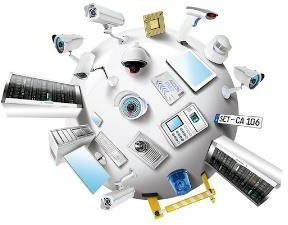
\includegraphics[width=\textwidth,height=0.55\textheight,keepaspectratio]{img/sl095.jpg}
\end{center}
\end{column}
\end{columns}
\end{frame}

\begin{frame}{Red Team}
\small
  \begin{itemize}
  \item Cuando nos encontramos en el entorno Wi-Fi las principales acciones que deberían ser realizadas son:
  
    \begin{itemize}
  \item Identificación de localizaciones objetivo (seleccionadas por diferencias).
  \item Identificación de redes Wi-Fi potenciales mediante Wigle.
  \item Identificación de localizaciones para el desarrollo de pruebas presenciales.
  \item Posteriormente será necesario desplazarse a las instalaciones para realizar el proceso de enumeración de redes y clientes Wi-Fi para identificar posibles vectores.
    \end{itemize}
  \end{itemize}
\end{frame}

\begin{frame}{Red Team}
\small
  \begin{itemize}
  \item En caso de tener que desarrollar pruebas sobre el ámbito físico, es recomendable que se obtenga la siguiente información preliminar:

    \begin{itemize}
  \item Identificación de localizaciones objetivo.
  \item Identificación de medidas de seguridad de forma pasiva (Google Maps).
  \item Identificación de zonas para el análisis/enumeración activa.
  \item Planteamiento de posibles vectores de ataque.
  \item Planteamiento de posibles vías de escape.
  \item Planteamiento de pretextos por si surgiera algún problema durante el desarrollo de pruebas activas en las localizaciones.
    \end{itemize}
  \end{itemize}
\end{frame}


\begin{frame}{Red Team}
\small
  \begin{itemize}
  \item Lockpicking
  \item Hay que recordar que este ámbito permite menos errores!
  \item Video muy recomendable sobre este tema: \href{https://www.youtube.com/watch?v=hngTacTVT3Y}{Video}
  \end{itemize}
\vfill
\begin{center}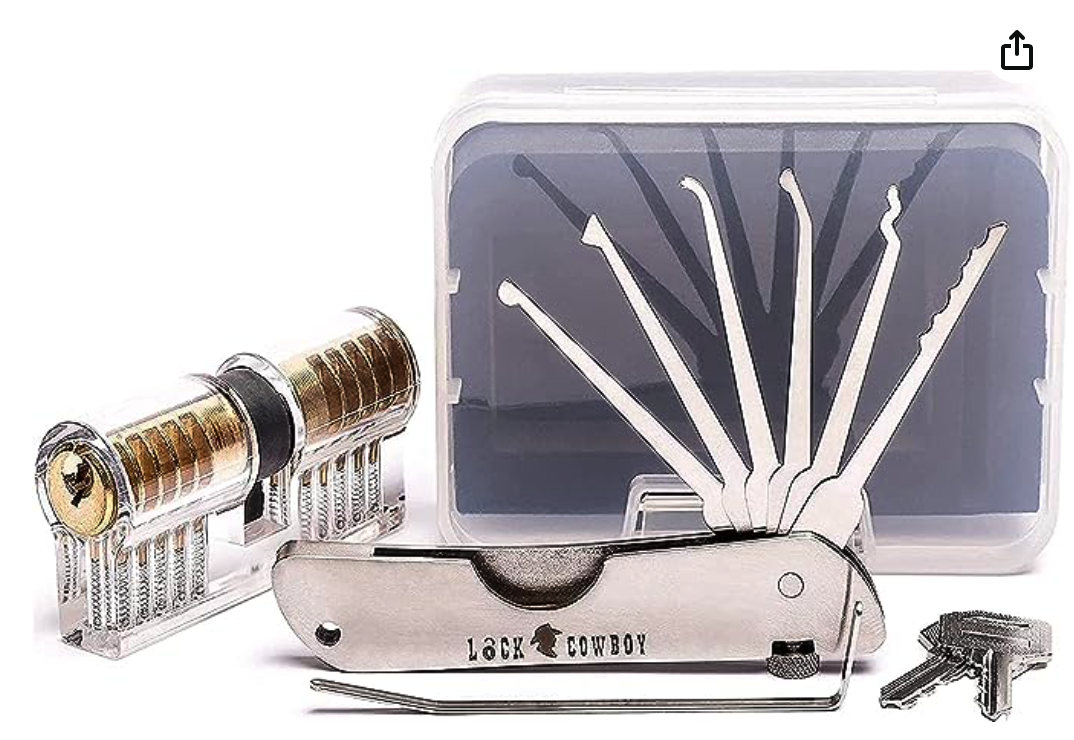
\includegraphics[width=0.62\textwidth,height=0.55\textheight,keepaspectratio]{img/sl098.png}
\end{center}
\end{frame}

\begin{frame}[allowframebreaks]{Red Team}
\small
  \begin{itemize}
  \item Si dentro del alcance se encuentra la posibilidad de realizar ataques de ingeniería social sobre los empleados, será necesario obtener al menos la siguiente información de manera previa a realizar las pruebas activas:
    \begin{itemize}

  \item Pre-análisis de la entidad y definición de posibles vectores.
  \item Identificación de perfiles de empleados.
  \item Identificación de empleados potencialmente objetivo.
  \item Desarrollo preliminar de pretextos.
  \item Desarrollo de planes de escape.
  \item Análisis y preparación de la interacción física o digital del ataque.
  \item Al igual que ocurre con el ámbito físico, aquí los intentos son limitados!
    \end{itemize}

  \end{itemize}
\end{frame}

\begin{frame}[allowframebreaks]{Red Team}
\small
  \begin{itemize}
  \item La ingeniería social también se puede aplicar a través de las redes sociales
  \item Información que se puede recoger mediante ingeniería social:
    \begin{itemize}
    \item Tarjetas de crédito, números de cuentas, DNIs, teléfonos
    \item Usuarios y contraseñas
    \item Productos de seguridad que se usan
    \item Sistemas operativos y versiones de software
    \item Información de red de la organización
    \item Direcciones IP de los servidores
      \item Un atacante puede averiguar una dirección IP enviando un mensaje vía Skype: \href{https://securityaffairs.com/150000/hacking/grabbing-ip-addr-via-skype-mobile-app.html}{noticia}
    \end{itemize}
  \end{itemize}
\end{frame}

\begin{frame}[allowframebreaks]{Red Team}
\small
  \begin{itemize}
  \item Por qué es relevante la ingenier´ia social en footprinting
  \item El atacante puede utilizar lainformación recopilada en fases anteriores (OSINT, LinkedIn, RRSS)
  \item Construye un pretexto creíble basado en datos reales de la víctima $\rightarrow$ Nombre, cargo, empresa, proyectos actuales, relaciones $\rightarrow$ todo obtenido de fuentes abiertas
  \item $\rightarrow$ La línea entre footprinting e ingeniería social es muy delgada: uno alimenta al otro
  \end{itemize}
\end{frame}

\section{OSINT}


\begin{frame}[allowframebreaks]{OSINT}
OSINT NO es recopilar información / enlaces y fragmentos de información, OSINT es análisis de inteligencia
\small
  \begin{itemize}
  \item Usos:
\begin{itemize}
  \item Reputación de usuarios
  \item Estudios sociológicos, psicológicos
  \item Auditoría
  \item Lanzamientos de ataques APT y spear phishing
  \end{itemize}
  \end{itemize}
\end{frame}

\begin{frame}{OSINT}
\footnotesize
\begin{columns}[c]
\begin{column}{0.70\textwidth}
  \begin{itemize}
  \item Requisitos: Se establecen todos los requerimientos que se deben cumplir, es decir, aquellas condiciones que deben satisfacerse para conseguir el objetivo.
  \item Fuentes de información: Identificar las fuentes de interés con información relevante, ya que hay que tener presente el volumen de información disponible en Internet y así optimizar el proceso.
  \item Adquisición: Se obtiene información a partir de las fuentes indicadas.
  \item Procesamiento: Consiste en dar formato (parsear) a toda la información recopilada de manera que posteriormente pueda ser analizada.
  \item Análisis: Se genera inteligencia a partir de los datos recopilados y procesados. El objetivo es relacionar la información de distintos orígenes buscando patrones que permitan llegar a una conclusión.
  \item Presentación de inteligencia: Consiste en presentar la información obtenida de una manera eficaz, potencialmente útil y comprensible, de manera que pueda ser explotada.
  \end{itemize}
\end{column}
\begin{column}{0.28\textwidth}
\begin{center}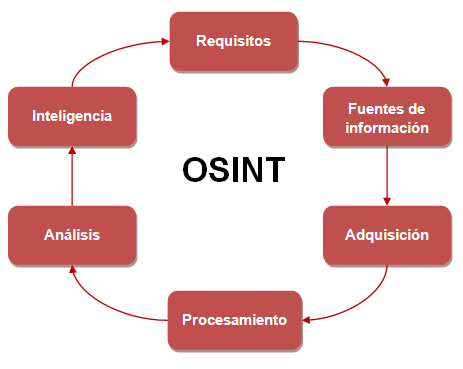
\includegraphics[width=\textwidth,height=0.6\textheight,keepaspectratio]{img/sl105.png}
\end{center}
\end{column}
\end{columns}
\end{frame}

\begin{frame}{OSINT}
\footnotesize
\begin{columns}[c]
\begin{column}{0.74\textwidth}
  \begin{itemize}
  \item Herramientas:
    \begin{itemize}
  \item \href{https://github.com/lanmaster53/recon-ng}{Recon-ng} (\href{https://www.youtube.com/watch?v=3_Uy_wex9xw}{ejemplo})
      \item \href{https://github.com/1aN0rmus/TekDefense-Automater}{Automater}
    \item \href{https://www.maltego.com/}{Maltego} (\href{https://ciberpatrulla.com/maltego/}{ejemplo})
    \item \href{https://github.com/i3visio/osrframework}{OSRFramework}
    \item \href{https://osintframework.com/}{OSINTframework}
    \item \href{https://github.com/DataSploit/datasploit}{Datasploit}
    \item \href{https://www.kitploit.com/2018/03/th3inspector-tool-for-information.html}{Th3inspector}
    \item \href{https://github.com/s0md3v/ReconDog}{Recon-Dog}
    \item \href{https://www.linkedin.com/posts/joan-moya-torremocha_informationsecurity-hacking-redteam-activity-7260626436930084864-Qou9/}{Ashok} (recon todo-en-uno: dorks, subdominios, puertos)
    \item \href{https://www.youtube.com/watch?v=nIpPHK0MJoU}{Golismero}
    \item \href{https://derechodelared.com/photon-mini-analisis-de-una-herramienta-osint/}{Photon}
    \item \href{https://www.hackplayers.com/2020/03/metabigor-osint-sin-api-keys.html}{Metabigor}
    \item \href{https://hakin9.org/reconspider-most-advanced-open-source-intelligence-osint-framework/}{Reconspider}
    \end{itemize}
  \item Distribución OSINT:
    \begin{itemize}
    \item \href{https://www.tracelabs.org/initiatives/osint-vm}{Trace Lab}
    \end{itemize}
  \end{itemize}
\end{column}
\begin{column}{0.24\textwidth}
\begin{center}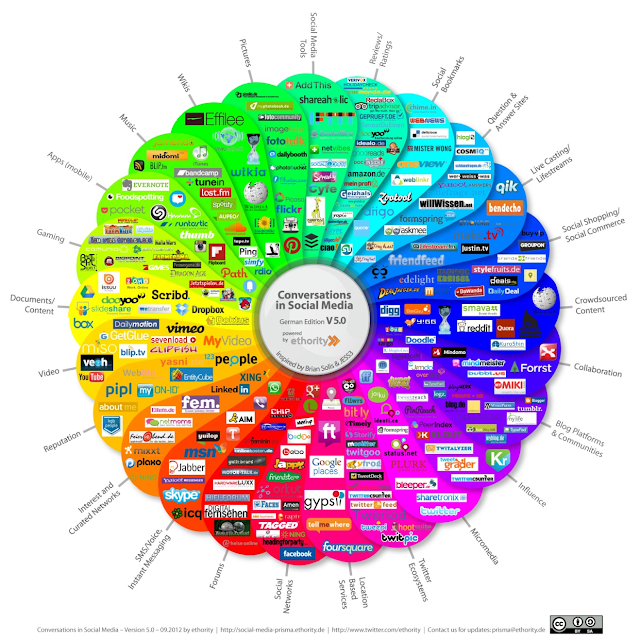
\includegraphics[width=\textwidth,height=0.6\textheight,keepaspectratio]{img/sl107.png}
\end{center}
\end{column}
\end{columns}
\end{frame}



\begin{frame}{OSINT}
\begin{center}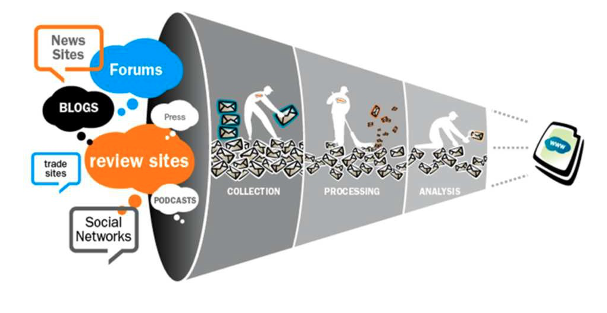
\includegraphics[width=\textwidth,height=0.82\textheight,keepaspectratio]{img/sl106.png}\end{center}
\end{frame}

\begin{frame}{OSINT}
\begin{center}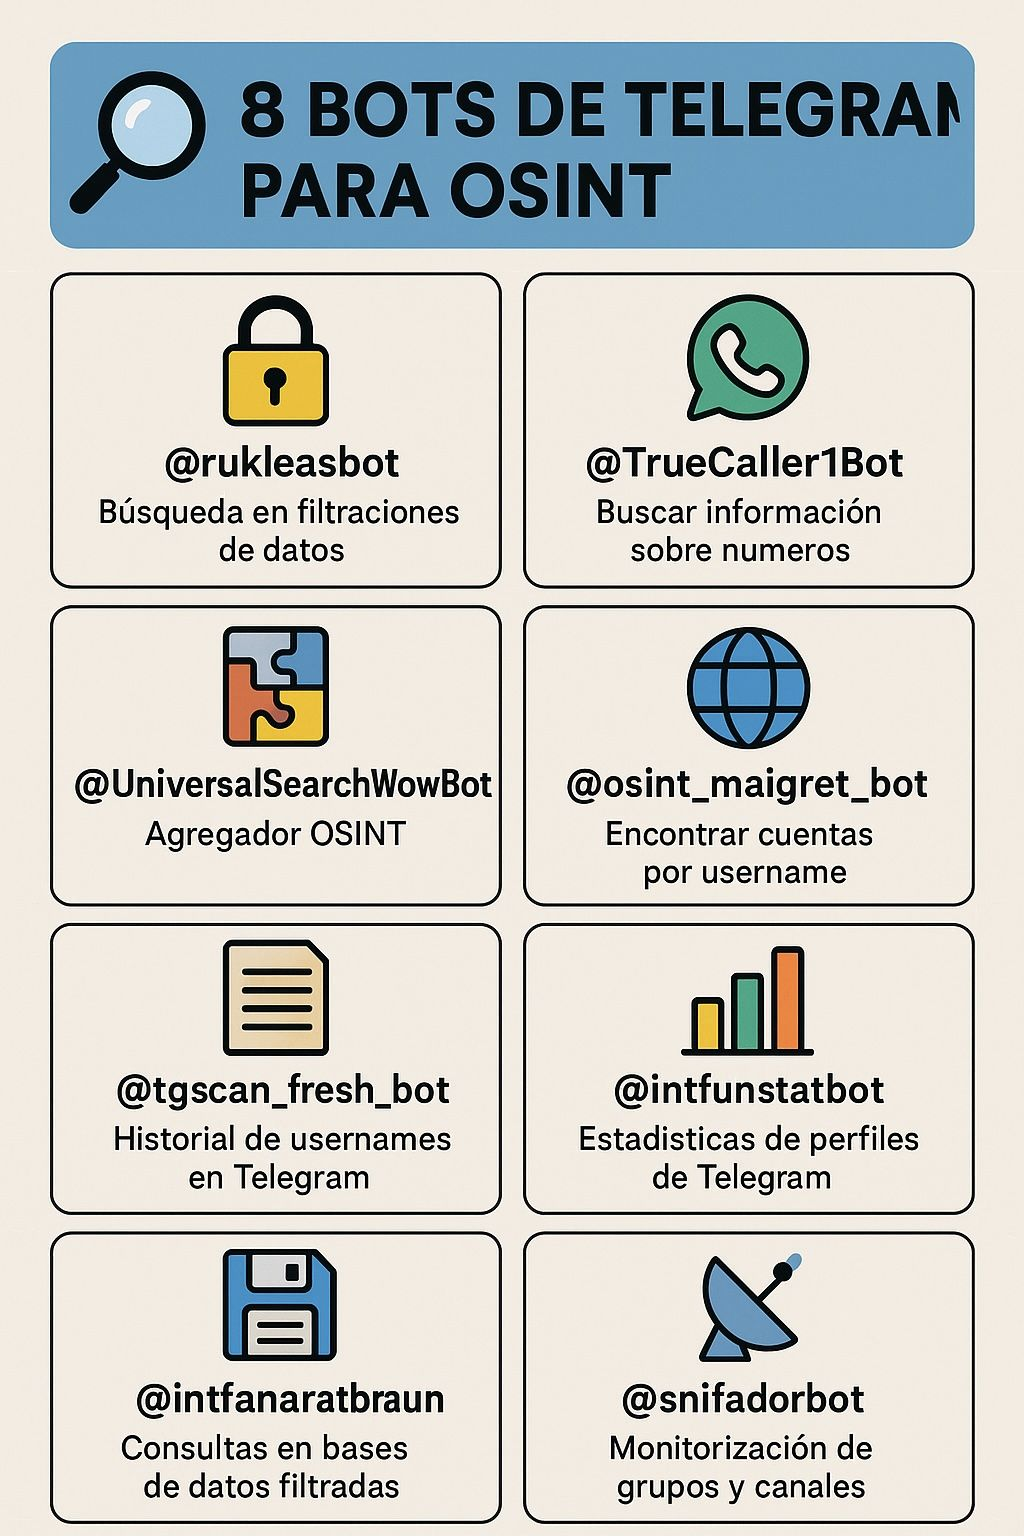
\includegraphics[width=0.55\textwidth,height=0.86\textheight,keepaspectratio]{img/sl108.jpg}\end{center}
\end{frame}

\begin{frame}[allowframebreaks]{OSINT}
\small
OSINT en la Práctica: El Caso Bellingcat
  \begin{itemize}
  \item Bellingcat es un colectivo internacional e independiente de periodismo de investigación. Investiga usando exclusivamente fuentes abiertas. 
  \item Casos emblemáticos:
  \begin{itemize}
  \item Derribo del vuelo MH17 --- Ucrania, 2014
  \begin{itemize}
  \item Localizaron el lanzador BUK mediante fotos y vídeos publicados en redes sociales
  \item Cruzaron metadatos EXIF con Google Maps, Yandex Panorama y vídeos de testigos
  \item $\rightarrow$ Identificaron la 53 Brigada rusa y la ruta completa del convoy con misil incluido
  \end{itemize}
  \item Identificación de agentes del GRU ruso --- Caso Skripal, 2018
    \begin{itemize}
  \item Partieron del número de pasaporte de los sospechosos (dato público en el juicio)
  \item Cruzaron bases de datos filtradas rusas, LinkedIn, redes sociales y registros de vuelo
  \item $\rightarrow$ Desvelaron identidades reales de agentes de inteligencia operando bajo identidades falsas
    \end{itemize}
  \item Técnicas OSINT empleadas:
      \begin{itemize}
  \item Geolocalización por sombras/edificios Búsqueda inversa de imágenes
  \item Metadatos EXIF Bases de datos públicas Registros de vuelo (FlightRadar24)
  \end{itemize}
\end{itemize}
\end{itemize}
\end{frame}

\begin{frame}{Ejercicio}
\small
\begin{center}
\includegraphics[width=0.45\textwidth,height=0.4\textheight,keepaspectratio]{img/sl111.jpg}
\end{center}
\vspace{0.5em}
  \begin{itemize}
  \item Serias capaz de realizar un ejercicio de OSINT con la herramienta Maltego frente a la organización objetivo
  \end{itemize}
\end{frame}


\section{Conclusiones}

\begin{frame}{Conclusiones}
\footnotesize
  \begin{itemize}
  \item El footprinting es la \textbf{primera fase} de cualquier auditoría o ejercicio de Red Team: sin un inventario correcto de activos, todas las fases posteriores (enumeración, explotación, post-explotación) trabajan sobre un alcance incompleto.
  \item La mayor parte del trabajo es \textbf{pasivo}: buscadores, dorks, certificados, registros públicos (whois, RIRs, DNS), filtraciones y metadatos. El objetivo se investiga \emph{sin tocarlo}, lo que hace esta fase prácticamente indetectable.
  \item La \textbf{superficie de exposición real} casi nunca coincide con la que la organización cree tener: subdominios olvidados, preproducción indexada, repositorios con credenciales, servicios expuestos en Shodan/Censys y documentos con metadatos son hallazgos habituales.
  \item El \textbf{factor humano} es un activo más: correos, perfiles en RRSS, cargos y contraseñas filtradas permiten construir pretextos creíbles. La frontera entre footprinting e ingeniería social es muy delgada; uno alimenta al otro.
  \item Recopilar datos no es OSINT. \textbf{OSINT es análisis de inteligencia}: correlacionar fuentes heterogéneas hasta obtener conclusiones accionables (metodología: requisitos $\rightarrow$ fuentes $\rightarrow$ adquisición $\rightarrow$ procesamiento $\rightarrow$ análisis $\rightarrow$ presentación).
  \item El proceso es \textbf{iterativo}: cada hallazgo (una IP, un ASN, un certificado, un empleado) abre nuevas ramas de búsqueda a las que hay que volver.
  \end{itemize}
\end{frame}

\begin{frame}{Conclusiones}
\footnotesize
Desde el punto de vista defensivo (Blue Team):
  \begin{itemize}
  \item Realizar footprinting \textbf{sobre uno mismo} de forma periódica: lo que encuentra un atacante también puede encontrarlo la organización, y antes.
  \item Higiene de la exposición: revisar dorks e indexación, robots.txt, mensajes de error, banners, repositorios públicos y limpiar metadatos antes de publicar documentos.
  \item Gestión del inventario: dominios, subdominios, certificados y rangos de red bajo control; dar de baja lo que ya no se usa (los activos huérfanos son el punto de entrada favorito).
  \item Protección del correo: \textbf{SPF, DKIM y DMARC} correctamente configurados para dificultar la suplantación del dominio.
  \item Monitorización continua: alertas sobre dominio y marca, vigilancia de filtraciones de credenciales y concienciación de los empleados sobre lo que publican.
  \end{itemize}
\vfill
\centering\textit{``El atacante solo necesita encontrar un activo olvidado; el defensor tiene que conocerlos todos.''}
\end{frame}



\begin{frame}[allowframebreaks]{Conclusiones}
\small
Flujo de trabajo del footprinting. De lo \textbf{pasivo} a lo \textbf{activo}, sin tocar (todavía) al objetivo:
  \begin{enumerate}
  \item \textbf{Alcance y objetivos}: dominios raíz, marcas, rangos e hipótesis; definir el alcance.
  \item \textbf{Huella pasiva}: buscadores y \emph{dorks}, filtraciones (HIBP, intelx), metadatos de documentos, RRSS y empleados (LinkedIn).
  \item \textbf{Infraestructura}: WHOIS/RDAP, ASN y rangos de red, DNS (registros, MX/NS), \textbf{Certificate Transparency} (crt.sh/Censys).
  \item \textbf{Subdominios y activos}: amass/subfinder/assetfinder + CT logs $\rightarrow$ resolver vivos (dnsx) y clasificar (Aquatone).
  \item \textbf{Tecnologías y exposición}: Shodan/Censys, \emph{hash} del favicon, \emph{fingerprinting} web, IP real tras WAF/CDN.
  \item \textbf{Correo}: SPF/DKIM/DMARC del dominio $\rightarrow$ ¿suplantable? (vector de phishing/BEC).
  \item \textbf{Consolidar}: inventario de activos + superficie de exposición; priorizar para la fase de enumeración/escaneo (tema 2.3).
  \end{enumerate}
\vfill
\footnotesize\textit{Regla de oro: cuanto más pasivo seas al principio, menos ruido generas y más difícil es que te detecten.}
\end{frame}

\begin{frame}[plain]
  \begin{center}
    {\Huge\bfseries\color{uznavy} ¡Gracias!}\\[1em]
    {\large Seguridad en Sistemas Informáticos --- Tema 2.1}
  \end{center}
\end{frame}

\pdfinfo{ /Title () /Author () /Subject () /Keywords () /Creator () /Producer () }
\end{document}

\begin{frame}[allowframebreaks]{Documentación complementaria \& Bibliografía}
\small
  \begin{itemize}
    \item \href{https://fwhibbit.es/harvey-v1-2-analisis-de-un-objetivo-parte-i}{Leer1} y \href{https://fwhibbit.es/harvey-v1-2-vigilancia-y-monitorizacion-en-twitter-parte-ii}{Leer2}
  \item \href{https://www.youtube.com/watch?v=1LLDS8fIW0A}{Video} y \href{https://www.youtube.com/watch?v=qwA6MmbeGNo}{Video}
    \begin{itemize}
    \item \href{https://www.youtube.com/watch?v=T8cLztvBClM}{Cómo los malos pueden conquistar el mundo con OSINT}
    \end{itemize}
  \item Ejercicios OSINT
    \begin{itemize}
    \item \href{https://fwhibbit.es/harvey-v1-2-analisis-de-un-objetivo-parte-i}{Leer1} y \href{https://fwhibbit.es/harvey-v1-2-vigilancia-y-monitorizacion-en-twitter-parte-ii}{Leer2}
    \end{itemize}
  \item Casos de Uso1: \href{http://www.elladodelmal.com/2017/01/odin-identificando-el-shadow-it-en-la.html}{parte1}, \href{http://www.elladodelmal.com/2017/01/odin-identificando-el-shadow-it-en-la_17.html}{parte2}, \href{http://www.elladodelmal.com/2017/01/odin-identificando-el-shadow-it-en-la_19.html}{parte3}
  \item Caso de Uso Maltego-1: \href{https://fwhibbit.es/introduccion-a-maltego}{parte1}, \href{https://fwhibbit.es/maltego-ii}{parte2}
  \item Caso de Uso Maltego-2: \href{https://www.elladodelmal.com/2010/08/mineria-de-datos-con-maltego-1-de-2.html}{parte1}, \href{https://www.elladodelmal.com/2010/09/mineria-de-datos-con-maltego-2-de-3.html}{parte2}, \href{https://www.elladodelmal.com/2010/09/mineria-de-datos-con-maltego-3-de-3.html}{parte3}
  \end{itemize}
\end{frame}

\begin{frame}[allowframebreaks]{Documentación complementaria \& Bibliografía}
OSINT: Recursos de Formación y Práctica
  \small
  \begin{itemize}
  \item \href{udemy.com/course/curso-avanzado-de-osint/}{Curso Udemy} --- Avanzado de OSINT (en español)
    \begin{itemize}

  \item Cubre herramientas y metodología OSINT de nivel avanzado
  \item Incluye módulos de RRSS, imágenes, metadatos, Deep Web y automatización
    \end{itemize}

  \item \href{bash-bunny.github.io/OSINTconLinux/}{OSINT con Linux} --- Guía práctica open source
      \begin{itemize}

  \item Repositorio con herramientas, scripts y técnicas organizadas por categoría
  \item Ideal como referencia rápida durante ejercicios de campo
      \end{itemize}

  
\end{itemize}
\end{frame}

\begin{frame}[allowframebreaks]{Documentación complementaria \& Bibliografía}
\small
  \begin{itemize}
  \item \href{https://pruebasaluuclm-my.sharepoint.com/personal/joseluis_martinez_uclm_es/_layouts/15/onedrive.aspx?id=\%2Fpersonal\%2Fjoseluis\%5Fmartinez\%5Fuclm\%5Fes\%2FDocuments\%2Fbiliografia\%2FVinny\%5FTroia\%2DHuntingCyber\%20Criminals\%2Epdf&parent=\%2Fpersonal\%2Fjoseluis\%5Fmartinez\%5Fuclm\%5Fes\%2FDocuments\%2Fbiliografia&ga=1}{Cazando ciber criminales}
  \item \href{https://ciberpatrulla.com/links/}{Ciberpatrulla}
  \item \href{http://index-of.co.uk/INFOSEC/La_Biblia_del_Footprinting.pdf}{La biblia del footprinting}
  \item \href{https://www.incibe.es/extfrontinteco/img/File/intecocert/EstudiosInformes/cert_inf_seguridad_information_gathering.pdf}{Incibe: Information Gathering}
  \item \href{https://i-intelligence.eu/uploads/public-documents/OSINT_Handbook_2020.pdf}{Open Source Intelligence}
  \item \href{http://www.vulnerabilityassessment.co.uk/Penetration\%20Test.html}{VulnerabilityAssement}
  \item \href{https://thehackerway.com/2020/05/24/20-servicios-online-interesantes-para-red-teaming-o-pentesting/amp/}{Herramientas online}
  \end{itemize}
\end{frame}

\begin{frame}{Ejercicio}
\small
\begin{center}
\includegraphics[width=0.45\textwidth,height=0.4\textheight,keepaspectratio]{img/sl111.jpg}
\end{center}
\vspace{0.5em}
   \href{https://labs.thehackerslabs.com/categories/5}{The Hackers Labs} --- 4 Retos OSINT
  \begin{itemize}

  \item Ejercicios prácticos diseñados para entrenar investigación OSINT real
  \item Nivel progresivo: desde búsqueda básica hasta geolocalización avanzada
  \item \href{https://thehackerslabs.com/libros/}{Libros}
  \item \href{https://thehackerslabs.com/post-it/}{Post-IT}
  \item \href{https://thehackerslabs.com/camara/}{Cámara}
  \item \href{https://thehackerslabs.com/phisermansphriends/}{PhisermanShiriends}
  \end{itemize}
\end{frame}



\begin{frame}[allowframebreaks]{Ejercicio}
Resuelve este laboratorio de hackthebox:
  \begin{itemize}
  \item \href{https://academy.hackthebox.com/module/details/112}{Ejercicio OSINT HackTheBox}
  \end{itemize}
\begin{center}
\includegraphics[width=0.72\textwidth,height=0.58\textheight,keepaspectratio]{img/sl113.jpg}
\end{center}
\end{frame}

\begin{frame}[allowframebreaks]{Ejercicio}
  \small
Realiza esta room en tryhackme sobre \href{https://tryhackme.com/room/threatinteltools}{threat intelligence}
  \begin{center}
\includegraphics[width=0.72\textwidth,height=0.58\textheight,keepaspectratio]{img/sl114.jpg}
\end{center}
\end{frame}

